\chapter{集成学习}
\label{chap:ensemble-learning}

信用风险模型可能利用不同的预测信息：线性模型概括全局趋势，决策树表达局部交互；两棵树也可能因训练样本不同而作出不同判断。将这些预测组合起来，有机会减少单个模型遗漏结构或受训练波动影响造成的误差。\term{集成学习}（ensemble learning）研究成员模型的生成与输出组合，并分析成员之间的依赖如何影响新样本预测。

组合收益取决于成员的预测误差及其共同部分。准确而互补的成员可能纠正彼此的错误，反复遗漏同一结构的成员则会保留共同误差。下文先定义成员输出与组合规则，再讨论三类训练机制：Bagging扰动训练过程后聚合成员，Boosting根据当前组合序贯增加修正，Stacking利用样本外预测学习组合。第\ref{sec:ensemble-evaluation}节进一步用误差分解和评价协议检验这些机制。

本章主要讨论监督预测，回归响应、类别标签、得分和概率分别采用前两章的任务与评价定义。无监督划分的组合见第\ref{sec:clustering-ensemble}节。对于分类投票，成员在带权分布下的学习能力控制训练误差，投票间隔及函数类条件再将训练表现联系到新样本风险（参考\BookSectionRef{sec:boosting}{第二卷“基础、理论和可信性”的“二分类学习的可学习性”章“集成学习”节}）。本章侧重成员生成、更新与组合，分别评价求解结果、样本外预测和计算成本。

\label{sec:ensemble-overview}

图\ref{fig:ensemble-three-mechanisms}在同一预测任务中比较成员的训练依赖。给定原训练数据后，Bagging成员可分别训练；Boosting的新成员使用前轮组合产生的修正信号；Stacking则在基成员之外增加一个由折外预测训练的组合层。依赖关系决定哪些计算可以并行，也决定二阶段训练需隔离哪些样本信息。

\begin{figure*}[htbp]
  \centering
  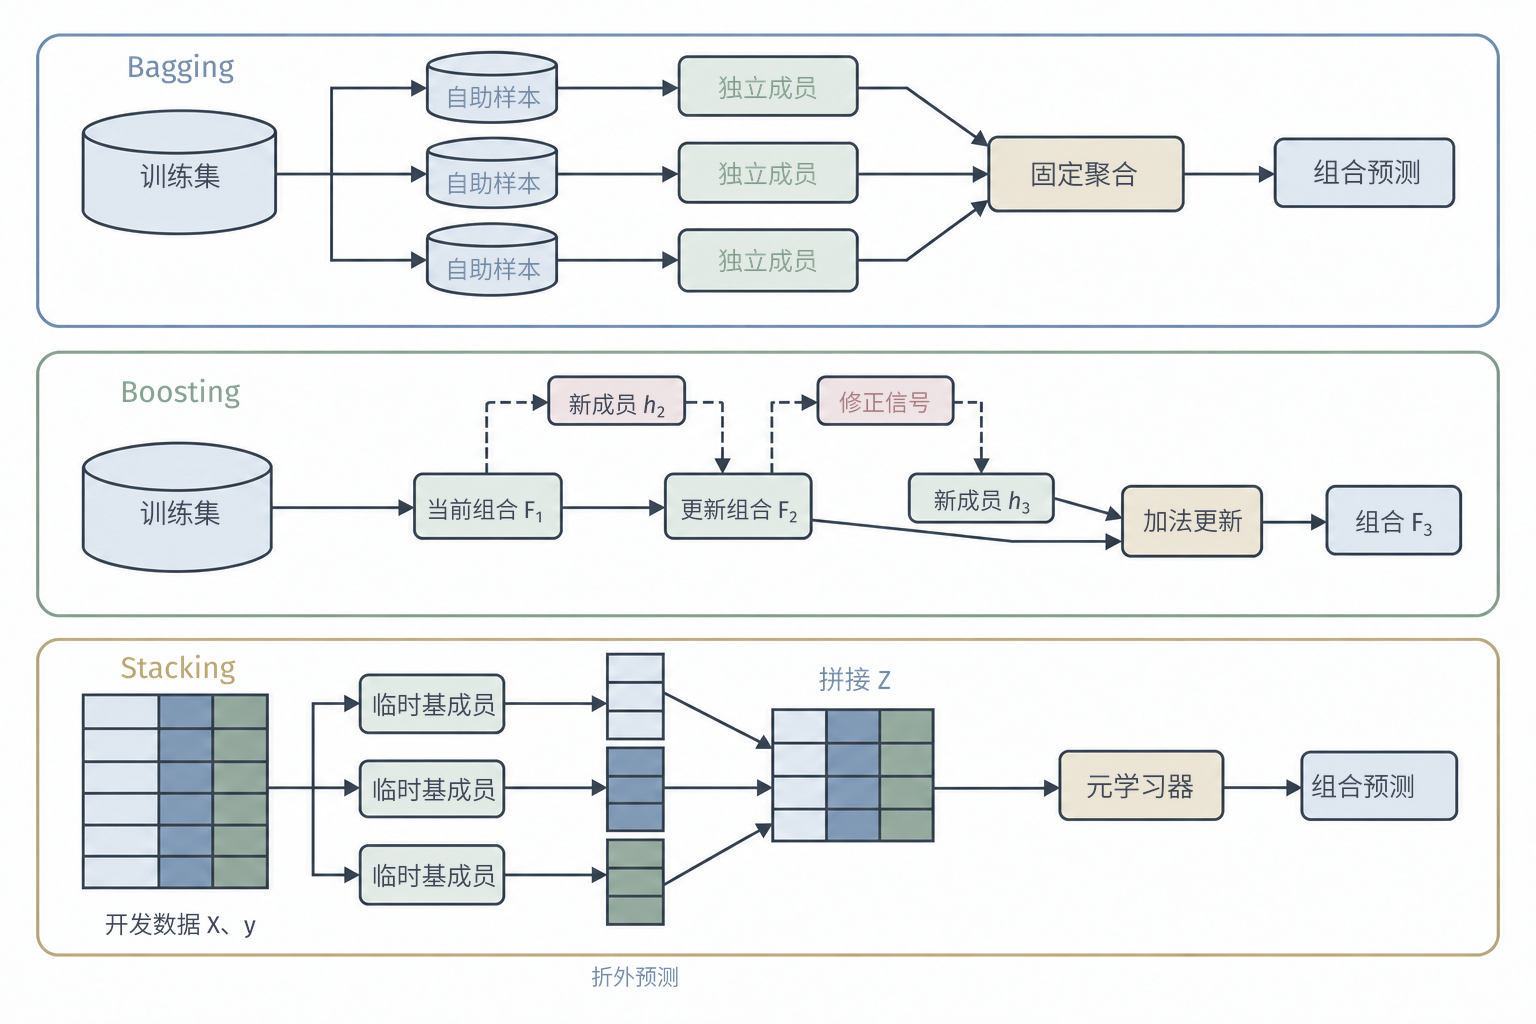
\includegraphics[width=130.048mm]{figures/03-models/01-classic-models/generated/ensemble-three-mechanisms/figure.png}
  \caption{Bagging、Boosting与Stacking的成员生成及组合关系。实线连接训练与预测步骤，虚线传递当前组合形成的修正信号。三类机制的成员依赖及组合规则不同；示意流程允许采用不同成员模型。}
  \label{fig:ensemble-three-mechanisms}
\end{figure*}

\paragraph{成员与组合输出}
\label{sec:ensemble-members-combination-output}

设训练集为
\[
  D_n=\{(\bm{x}_i,y_i)\}_{i=1}^{n},
\]
学习过程产生$M$个\term{成员模型}$h_1,\ldots,h_M$。用$\mathcal{C}$表示组合规则，\term{集成模型}的预测统一写成
\begin{equation}
  H(\bm{x})
  =\mathcal{C}\bigl(h_1(\bm{x}),\ldots,h_M(\bm{x})\bigr).
  \label{eq:ensemble-combination}
\end{equation}
式\eqref{eq:ensemble-combination}将成员预测映射为最终输出，具体规则由预测对象确定。回归成员若都预测同一个数值目标，可以采用等权平均
\[
  H(\bm{x})=\frac{1}{M}\sum_{m=1}^{M}h_m(\bm{x}),
\]
也可以用非负权重$w_m$作加权平均，其中$\sum_m w_m=1$。分类成员则可能输出硬标签、类别得分或类别概率。硬标签对应类别投票，同尺度得分或同类概率可逐类平均后决策；混合不同输出前，需要把它们转换为含义一致的量。

组合之前需要明确输出的数值含义。直接平均不同尺度的分类得分，会使数值范围较大的成员占据更大作用；平均类别概率则保持概率向量形式，其校准仍由新样本上的频率对应关系评价。元学习器若把得分转换为概率，这一映射也属于需要验证的模型。第\ref{sec:classification-evaluation}节分别给出了标签、排序与概率的评价方法。

权重的确定方式构成组合模型的一部分。等权平均固定每个成员的贡献，AdaBoost在序贯更新中估计贡献，线性Stacking根据折外预测学习权重。权重还可以依赖输入，此时$w_m=w_m(\bm{x})$，不同样本会调用不同成员或采用不同组合比例。成员数量、权重约束、组合层复杂度以及是否允许输入相关组合，都属于训练或验证流程需要确定的模型选择。


\section{基于Bagging的集成}
\label{sec:ensemble-bagging}

决策树的上层分裂可能随少量训练记录变化而改变，预测也随之波动。对同一总体的多份训练集分别建模并平均，可以削弱其中不共享的波动；实际通常只有一份数据，因而需要近似这种重复训练。\term{装袋法}（bootstrap aggregating, Bagging）用自助采样从现有训练集构造多份样本，分别训练成员，再用固定规则聚合。重采样使训练波动转为成员差异，固定聚合再削弱其中部分变化；成员共享的表示偏差则继续保留\scite{breiman1996bagging}。

\subsection{Bagging}
\label{sec:ensemble-bagging-bootstrap}

\subsubsection{自助样本与聚合预测}

对第$m$个成员，从$\{1,\ldots,n\}$中独立、等概率、有放回地抽取$n$次索引，所得多重集合记为$I^{(m)}$。有放回抽样使部分记录重复进入成员训练，也使部分记录留在该成员之外。学习算法$\mathcal{A}$在相应自助样本上训练出
\[
  h_m=\mathcal{A}\!\left(D_n^{(m)}\right),
  \qquad
  D_n^{(m)}=\{(\bm{x}_i,y_i):i\in I^{(m)}\}.
\]
回归通常平均$h_m(\bm{x})$；分类可以投票，也可以在成员输出具有同一语义时平均逐类得分或概率。可以改变自助样本大小或采用其他成员算法。此时仍需检验重采样是否使成员在新样本上产生互补预测。

一份大小为$n$的标准自助样本没有抽中原始样本$i$的概率为
\begin{equation}
  \mathbb{P}\!\left(i\notin I^{(m)}\right)
  =
  \left(1-\frac{1}{n}\right)^n
  \longrightarrow e^{-1}.
  \label{eq:ensemble-oob-probability}
\end{equation}
因此，每个成员平均约有$36.8\%$的原始样本未参与其训练。这些样本构成该成员的\term{袋外样本}（out-of-bag sample, OOB sample）。反过来，对每个训练样本$i$，可以只收集没有使用它训练的成员预测。令
\[
  \mathcal{M}_{i}^{\mathrm{OOB}}
  =\{m:i\notin I^{(m)}\},
\]
当$\mathcal{M}_{i}^{\mathrm{OOB}}$非空时，回归的袋外预测可写为
\begin{equation}
  \widehat{y}_{i}^{\mathrm{OOB}}
  =
  \frac{1}{|\mathcal{M}_{i}^{\mathrm{OOB}}|}
  \sum_{m\in\mathcal{M}_{i}^{\mathrm{OOB}}}h_m(\bm{x}_i),
  \label{eq:ensemble-oob-prediction}
\end{equation}
分类则对同一成员集合投票或平均类别输出。图\ref{fig:ensemble-bagging-oob}按样本收集符合条件的成员：每个样本的袋外预测由其未参与训练的成员子集给出，子集随样本变化。

\begin{figure*}[htbp]
  \centering
  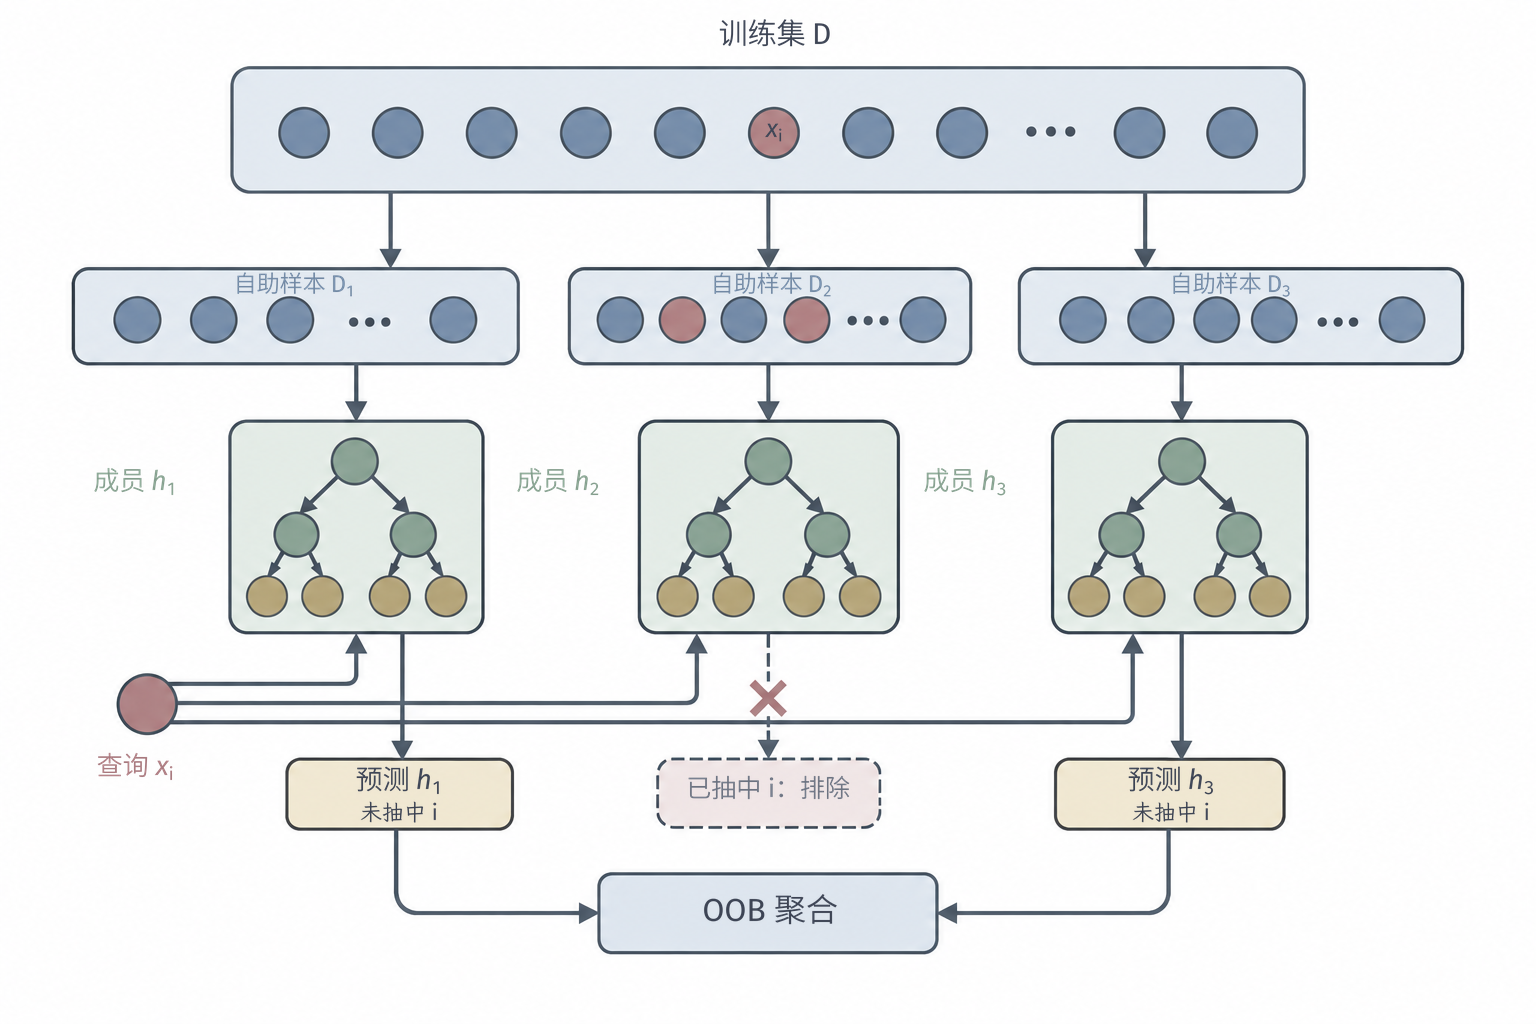
\includegraphics[width=130.048mm]{figures/03-models/01-classic-models/generated/ensemble-bagging-oob/figure.png}
  \caption{Bagging训练与袋外预测。每个成员只使用其自助样本训练；对训练样本$\bm{x}_i$，袋外预测只聚合未抽中$i$的成员。索引与集合展示样本和成员的对应关系；成员数有限时，各样本得到的袋外预测数量不同。}
  \label{fig:ensemble-bagging-oob}
\end{figure*}

\subsubsection{成员数量与误差来源}

给定原数据后，独立的重采样及训练可分配给不同计算单元。评价并行收益时，需要同时计入总工作量与实际经过时间：若单个成员的训练和预测成本分别为$C_{\mathrm{train}}$与$C_{\mathrm{pred}}$，朴素实现的总工作量仍约随$M C_{\mathrm{train}}$和$M C_{\mathrm{pred}}$增长。模型存储也通常随成员数量增加。

在固定训练集上增加独立随机成员，主要减少有限次抽样的Monte Carlo误差；等权平均逐渐逼近该随机训练机制的期望预测。原数据的抽样误差和模型失配仍影响这一期望，共同误差也会留在组合中。实践中可以观察袋外损失随成员数的变化，在曲线趋于稳定后停止增加成员，但这个停止规则也属于模型选择过程。

单树复杂度控制每份样本上的拟合，树数控制随机预测的平均程度。较深树可以表达更细的分区，也可能对扰动更敏感；叶规模与深度限制则可减少极小叶和噪声标签的影响。叶最小样本量、最大深度、类别权重和自助样本大小仍须与成员数共同选择，尤其在标签噪声、极小叶或类别极不平衡时。

\subsubsection{袋外预测的用途与边界}

袋外预测使当前标签与产生该预测的成员训练分离，可用于绘制树数—损失曲线、内部误差估计和置换重要性。可用成员数随机变化，自助训练集又相互重叠，这一数据结构与固定折的交叉验证不同。成员数很小时，某些样本可能没有足够的袋外预测。

反复用袋外结果选择结构、树数或特征处理，会使袋外误差成为开发证据；最终冻结流程需要另用测试数据评价。时间序列、分组样本或空间相关数据还要求自助抽样尊重依赖单位；逐行重采样会破坏原有数据结构。袋外结果的解释还依赖抽样单位与未来使用的数据制度。

\subsection{随机森林}
\label{sec:ensemble-random-forest}

树Bagging改变样本，却可能保留相同的强特征和上层分裂；这些共同选择使成员预测继续相关。\term{随机森林}（random forest）在树的自助采样之外加入节点级特征随机化：每个节点先随机抽取一组候选特征，再只在这组特征中搜索分裂。树仍按第\ref{sec:regression-trees}节或第\ref{sec:classification-trees}节的任务准则形成叶输出，改变的是每个成员可参与分裂搜索的信息\scite{breiman2001randomforests}。

节点候选特征数同时影响单树可用的信息和不同树的分裂差异。候选数接近全部特征时，森林更接近普通的树Bagging；候选数较小时，不同树更可能采用不同分裂，但单棵树也更容易错过当前节点上的有效特征。合适的候选规模取决于特征冗余、样本量和树深，可在固定验证协议下比较。

固定训练集并增加树数，可以减少森林平均预测的随机波动；所得极限仍由当前样本及树构造决定。总体风险另外受分布与估计条件控制，更多树也继续消耗存储和推理计算。随机森林的一致性结论通常针对特定的树构造、抽样比例与分布条件；实际软件在缺失值、类别特征、停止规则和并行实现上的差异，可能不满足同一组理论假设\scite{scornet2015consistency}。

\subsubsection{特征重要性的解释}

树集成常附带两类特征重要性。\term{不纯度下降重要性}（impurity-decrease importance）累计某个特征参与分裂时带来的加权目标下降，计算方便，却可能偏向候选切分较多的特征。相关变量可以在分裂中相互替代，累计下降反映实际选中的路径，因而与变量的独立贡献不同。

\term{置换重要性}（permutation importance）固定已训练模型，在评价数据上打乱一个特征，再观察预测损失增加多少。这个量直接对应已拟合模型在所选扰动下对该特征的依赖，但打乱会破坏该特征与其他特征的联合关系。高度相关的特征可能互相替代，使单个特征的置换影响看起来很小；不现实的特征组合也可能夸大损失变化。这些量分别描述训练分裂和预测扰动中的模型依赖，解释时需说明评价数据、损失及置换方式；因果判断另需因果假设与证据\scite{strobl2007bias}。

图\ref{fig:ensemble-tree-randomization}沿一棵树的构造路径比较三种随机化位置。树Bagging主要改变成员看到的训练样本；随机森林还在每个节点抽取候选特征；Extra Trees继续把随机性放入候选阈值。三者继续以任务准则比较分裂，差别在于进入贪心搜索的样本、特征和阈值。

\begin{figure*}[htbp]
  \centering
  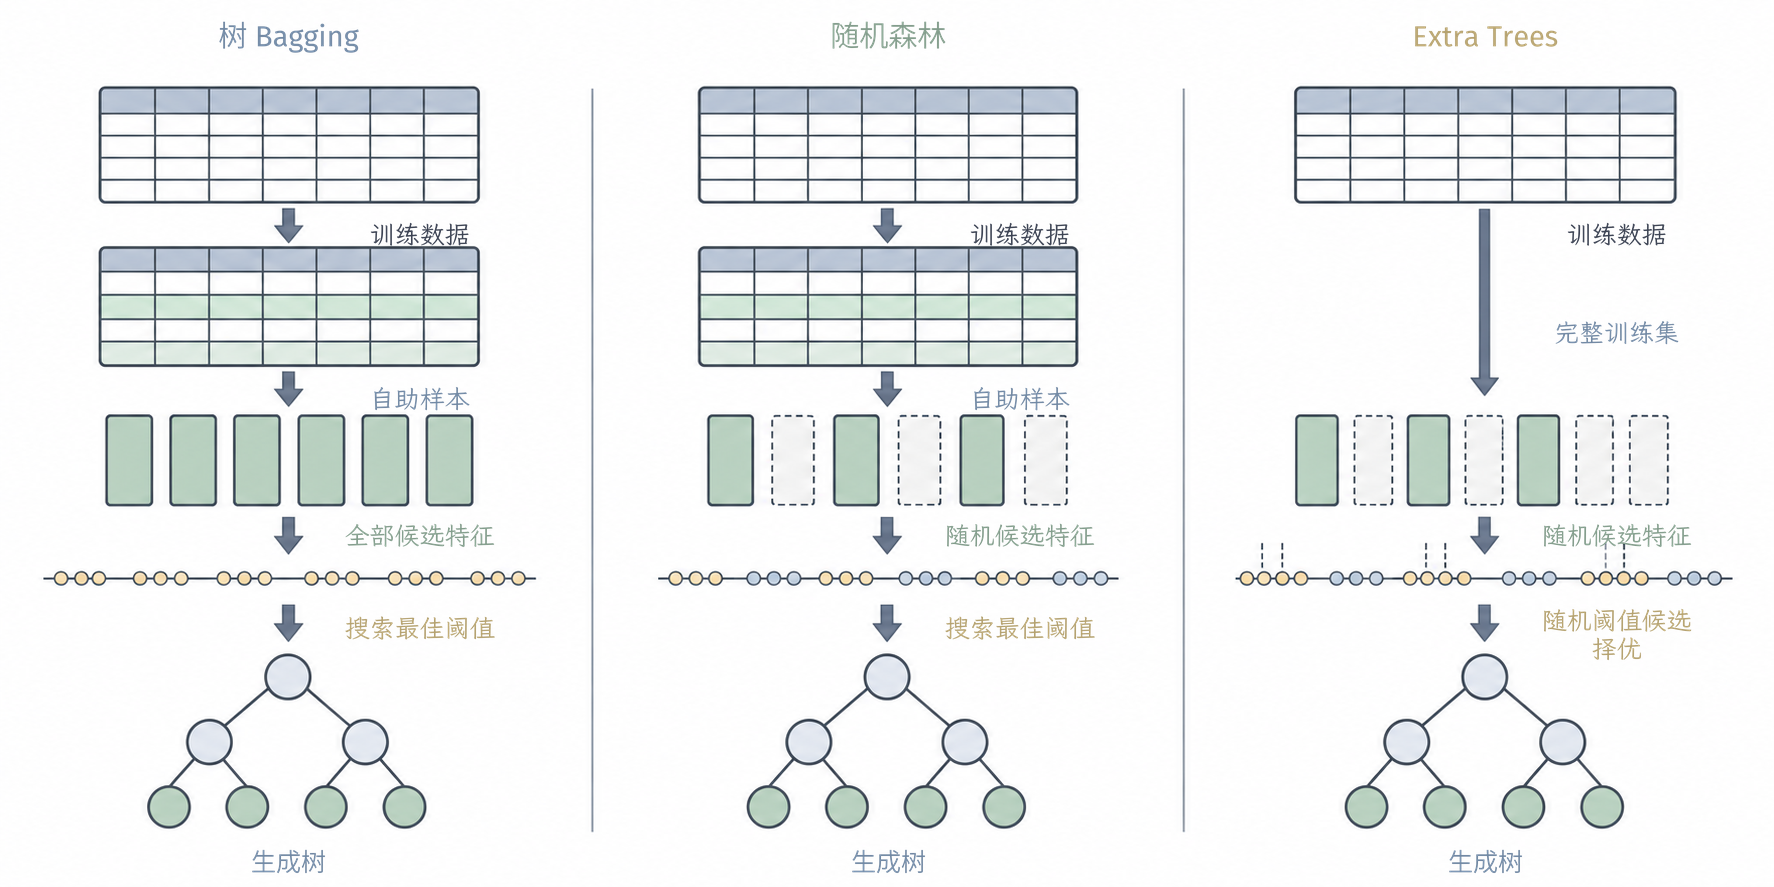
\includegraphics[width=150.199mm]{figures/03-models/01-classic-models/generated/ensemble-tree-randomization/figure.png}
  \caption{树Bagging、随机森林与Extra Trees的随机化位置。每栏从样本来源出发，依次展示候选特征、候选阈值与成员树；候选选择中的随机性和任务准则约束分别标在相应步骤。每栏首框直接标出训练样本来源：前两栏采用自助采样，Extra Trees栏采用原始方法的完整训练集设定；具体实现也可能额外启用自助采样。}
  \label{fig:ensemble-tree-randomization}
\end{figure*}

\subsection{极度随机树（Extra Trees）}
\label{sec:ensemble-extra-trees}

随机森林已随机选择候选特征，阈值仍通过当前节点的数据搜索。\term{极度随机树}（extremely randomized trees, Extra Trees）把随机性进一步放入阈值选择：在每个节点，对随机选出的候选特征生成随机切分点，再从这些随机候选中选择得分较好的切分。原始方法通常让各棵树使用完整训练集，把成员差异主要交给特征与阈值随机化；具体软件也可能允许额外使用自助采样\scite{geurts2006extra}。

随机阈值减少了穷举候选切分的工作，也会让单棵树偏离当前样本上的最佳贪心分裂。组合是否改善，取决于单树预测能力下降与成员依赖减弱之间的平衡。候选特征数、每个特征的随机阈值数、叶最小样本量以及是否采用自助采样共同决定这个平衡；增加随机化能否降低测试损失，需要在同一数据与预算下检验。

这些扩展可从“扰动发生在哪里”比较：在本节的宽泛机制分类中，样本、特征或阈值扰动都用于产生可独立训练的成员，再按固定规则聚合。标准Bagging则特指自助采样聚合。随机子空间只扰动成员可见的特征，Pasting以无放回子样本替代自助样本，随机权重则让同一记录在不同成员中具有不同影响。改变扰动方式后，袋外预测的可用条件也随是否采用自助采样而变化。

\subsection{模型对比与总结}
\label{sec:ensemble-bagging-comparison}

表\ref{tab:ensemble-bagging-comparison}固定树为成员，比较三种方法怎样产生差异。普通Bagging只改变训练样本；随机森林再限制节点可见的候选特征；Extra Trees进一步随机化候选阈值。三种方式还可能采用不同抽样方案，单树误差和搜索成本需与成员依赖一起比较。

\begin{table*}[htbp]
  \centering
  \small
  \begin{tabularx}{\linewidth}{@{}>{\raggedright\arraybackslash}p{24mm}*{6}{>{\raggedright\arraybackslash}X}@{}}
    \toprule
    方法 & 样本扰动 & 节点候选特征 & 阈值选择 & 袋外预测 & 成员训练 & 主要边界 \\
    \midrule
    树Bagging & 通常自助采样 & 全部特征 & 在候选中搜索 & 标准自助设定下可用 & 成员间可并行 & 强特征可能使树高度相关 \\
    随机森林 & 通常自助采样 & 随机特征子集 & 在子集内搜索 & 标准自助设定下可用 & 成员间可并行 & 候选数过小会削弱单树 \\
    Extra Trees & 原始方法使用完整训练集；实现可选自助采样 & 随机特征子集 & 生成随机阈值后择优 & 仅在采用自助采样时可用 & 成员间可并行 & 过强随机化会增大单树误差 \\
    \bottomrule
  \end{tabularx}
  \caption{以树为成员时，Bagging、随机森林与Extra Trees的机制比较。表中列出基本构造；比较具体实现时，还需记录抽样设置，并固定树复杂度、成员数和计算预算。}
  \label{tab:ensemble-bagging-comparison}
\end{table*}

Bagging先产生训练差异，再聚合预测以削弱部分波动。固定聚合保留成员共享的遗漏；若希望让新成员针对这些不足训练，就需要根据当前组合产生修正信号。下一节据此转向序贯提升。

\section{基于Boosting的集成}
\label{sec:ensemble-boosting}

Bagging分别训练成员后才聚合；如果希望新成员针对当前预测误差学习，就需要先计算已有组合的输出。\term{Boosting}（提升）构造一个序贯加法模型：第$t$轮先观察已有函数$F_{t-1}$，再选择新成员及其贡献，以降低指定训练目标。AdaBoost、梯度提升及现代提升树共享这种依赖关系，但它们生成修正信号和近似目标的方式不同。

\subsection{前向逐步加法模型}
\label{sec:ensemble-stagewise-additive}

设$F_0$为初始预测，Boosting经过$T$轮得到
\begin{equation}
  F_T(\bm{x})
  =
  F_0(\bm{x})
  +
  \sum_{t=1}^{T}\alpha_t h_t(\bm{x}),
  \label{eq:ensemble-additive-model}
\end{equation}
其中$h_t$是第$t$个成员，$\alpha_t$控制其贡献。为使复杂度惩罚对应真正加入模型的函数，把本轮增量记为$f_t=\alpha_t h_t$。给定损失$\ell$，理想化的第$t$轮直接优化增量：
\begin{equation}
  f_t
  \in
  \argmin_{f\in\mathcal{F}}
  \sum_{i=1}^{n}
  \ell\!\left(
    y_i,
    F_{t-1}(\bm{x}_i)+f(\bm{x}_i)
  \right)
  +\Omega_t(f).
  \label{eq:ensemble-forward-stagewise}
\end{equation}
这里$\mathcal{F}=\{\alpha h:\alpha\in\mathbb{R},h\in\mathcal{H}\}$是由成员函数族$\mathcal{H}$生成的增量函数族，$\Omega_t$是相应复杂度惩罚，也可以取零。

树的叶数惩罚控制分区规模，叶输出范数惩罚控制本轮增量。范数应作用于$f$，使惩罚随实际加入组合的幅度变化；若仅惩罚$h$，它与$\alpha$的相互缩放会改变惩罚却保持预测。

逐步优化固定已有成员，减少了联合搜索变量，但最优范围仅限本轮增量。后文用梯度拟合、二阶目标和收缩构造近似更新。

不同方法将当前预测转换为不同的训练信号。AdaBoost改变训练样本的权重，使当前错分记录在下一轮具有更大影响；梯度提升把损失对当前预测的负梯度作为伪响应；二阶提升树还利用局部曲率近似叶权重和分裂收益。平方损失的负梯度恰为普通响应残差，其他损失则给出不同修正量。损失决定了下一轮成员拟合的对象。

\subsection{AdaBoost}
\label{sec:ensemble-adaboost}

\term{AdaBoost}（adaptive boosting）通过更新样本权重，使新分类器更多地处理当前组合反复错分的记录。考虑二分类标签$y_i\in\{-1,1\}$和成员$h_t(\bm{x})\in\{-1,1\}$。初始样本权重为$w_i^{(1)}=1/n$，第$t$轮成员的加权错误率为
\begin{equation}
  \epsilon_t
  =
  \sum_{i=1}^{n}
  w_i^{(t)}
  \mathbb{I}\!\left\{y_i\neq h_t(\bm{x}_i)\right\}.
  \label{eq:ensemble-adaboost-error}
\end{equation}
当$0<\epsilon_t<1/2$时，成员投票权重取
\begin{equation}
  \alpha_t
  =
  \frac{1}{2}
  \log\frac{1-\epsilon_t}{\epsilon_t},
  \qquad
  w_i^{(t+1)}
  =
  \frac{
    w_i^{(t)}
    \exp\!\left[-\alpha_t y_i h_t(\bm{x}_i)\right]
  }{Z_t},
  \label{eq:ensemble-adaboost-update}
\end{equation}
其中$Z_t$使新权重和为1。错分样本满足$y_i h_t(\bm{x}_i)=-1$，权重乘上$e^{\alpha_t}$；正确样本的权重乘上$e^{-\alpha_t}$。

若$\epsilon_t=0$，在这些正权重下当前成员已分对全部训练样本，便直接输出$h_t$并停止，避免将发散系数代入更新（参考\BookSectionRef{sec:boosting}{第二卷“基础、理论和可信性”的“二分类学习的可学习性”章“集成学习”节}）。其余情况下，最终分类器在预先固定平局规则后按$\operatorname{sign}(\sum_t\alpha_t h_t(\bm{x}))$决策。正的成员贡献要求当前加权错误率小于$1/2$；条件未满足时，可停止本轮、调整训练或采用相应变体。

图\ref{fig:ensemble-adaboost-weight-update}将分类错误与下一轮权重连接起来。当前分类结果先改变样本权重，再由归一化后的权重决定下一轮成员看到的训练分布；错分记录因而获得更大的后续影响。

\begin{figure*}[htbp]
  \centering
  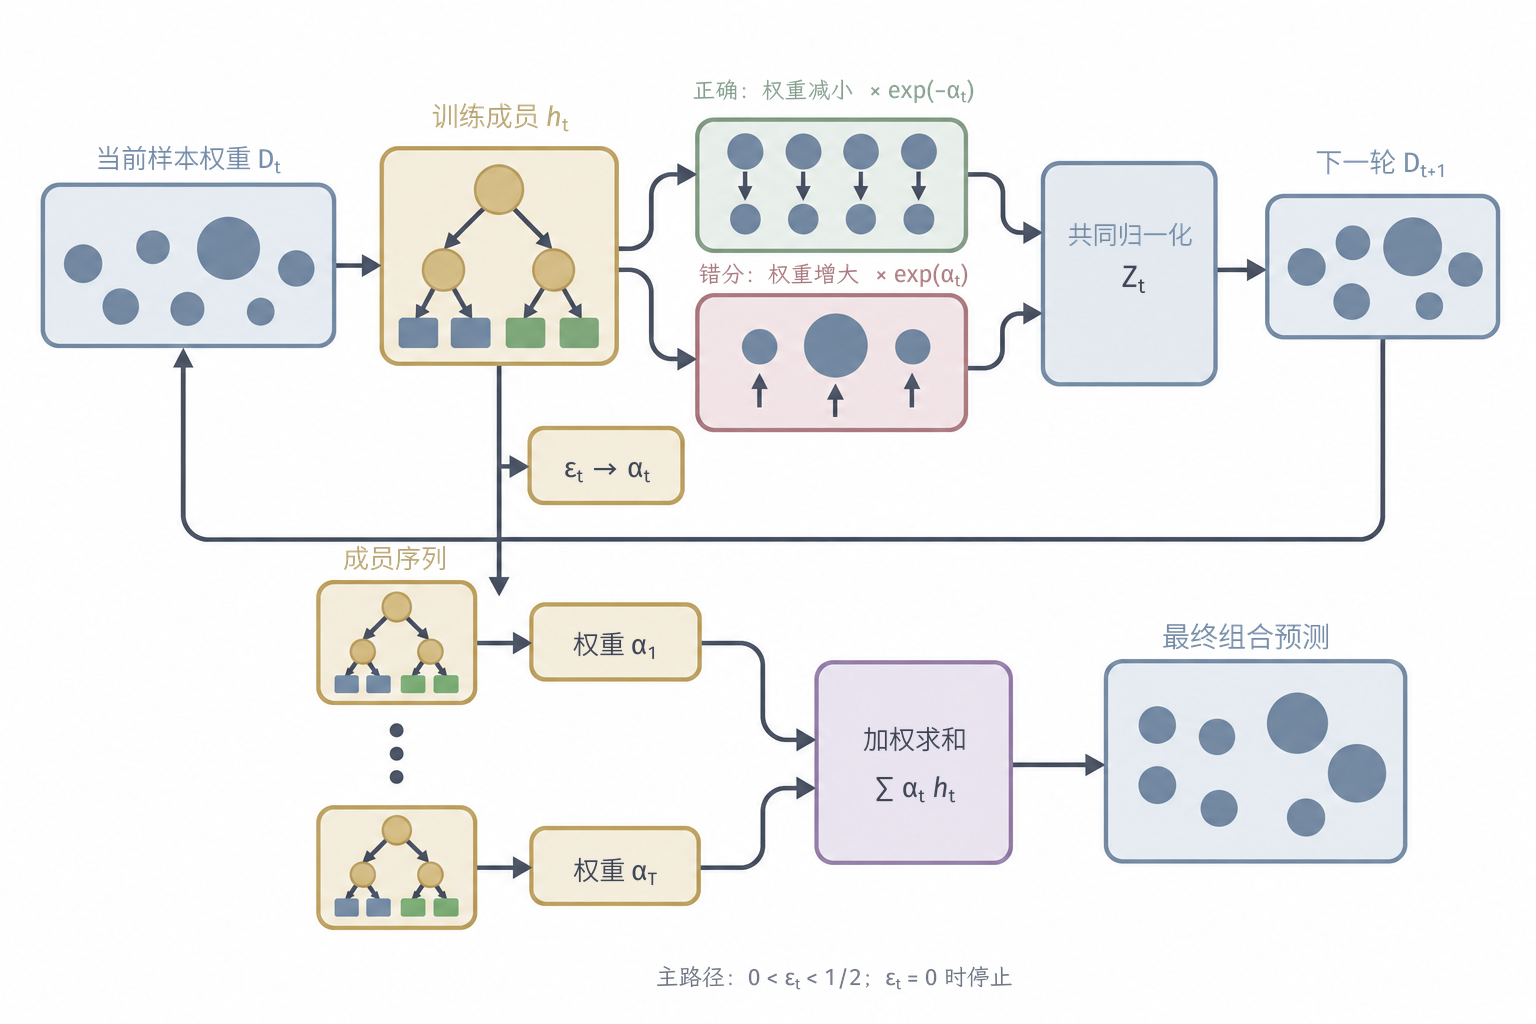
\includegraphics[width=130.048mm]{figures/03-models/01-classic-models/generated/ensemble-adaboost-weight-update/figure.png}
  \caption{AdaBoost的样本权重更新。分类结果把样本分成正确与错分两路，两路缩放后的权重汇合并归一化，形成下一轮训练分布。实线表示常规训练与正确分类样本的更新路径，红色虚线强调错分样本被放大的路径。}
  \label{fig:ensemble-adaboost-weight-update}
\end{figure*}

这一更新也可以从指数损失解释。令$F(\bm{x})=\sum_t\alpha_t h_t(\bm{x})$，经验目标为
\[
  \sum_{i=1}^{n}\exp\!\left[-y_iF(\bm{x}_i)\right].
\]
固定$F_{t-1}$后选择$h_t$与$\alpha_t$，在$0<\epsilon_t<1/2$时可以导出式\eqref{eq:ensemble-adaboost-update}。样本重加权由指数损失的逐步优化导出，因此其作用可以通过该目标分析\scite{freund1997boosting,friedman2000adaboost}。

持续错分的记录获得更大权重，后续成员因而可能恢复稀少的边界结构，也可能追逐错误标签。若成员在每轮带权分布下都优于随机猜测，可以控制训练错误的下降；新样本风险还与投票间隔和函数类条件有关（参考\BookSectionRef{sec:boosting}{第二卷“基础、理论和可信性”的“二分类学习的可学习性”章“集成学习”节}）。实际训练需同时检查错误记录的来源、训练目标和独立测试表现。

多分类AdaBoost需要重新定义成员错误与类别得分，回归变体则要用响应误差决定样本权重和预测聚合。这些变体沿用序贯重加权，但成员错误、系数与聚合需要按各自任务重新推导。评价分别采用分类或回归的输出和损失。

\subsection{梯度提升机与GBDT}
\label{sec:ensemble-gradient-boosting}

改变任务损失后，也需要改变修正信号。对于关于预测可微的损失，其负梯度指出当前预测降低经验目标的方向。\term{梯度提升机}（gradient boosting machine, GBM）用基学习器逼近这个负梯度方向，从而把序贯加法扩展到更一般的损失\scite{friedman2001gradientboost}。

通常从使训练损失最小的常数预测开始：
\begin{equation}
  F_0(\bm{x})=c_0,
  \qquad
  c_0\in\argmin_c\sum_{i=1}^{n}\ell(y_i,c).
  \label{eq:ensemble-gbm-initialization}
\end{equation}
平方损失下$c_0$是响应均值。这里要求存在有限的最小化点；若某种损失与数据组合使最优常数趋于无穷，就需约束预测范围或另定有限初始化。

在第$t$轮，对每个训练样本计算\term{伪残差}（pseudo-residual），即损失在当前预测处的负导数：
\begin{equation}
  r_i^{(t)}
  =
  -
  \left.
  \frac{\partial \ell(y_i,z)}{\partial z}
  \right|_{z=F_{t-1}(\bm{x}_i)}.
  \label{eq:ensemble-pseudo-residual}
\end{equation}
随后用平方误差把这些修正量拟合到成员函数族：
\begin{equation}
  h_t\in\argmin_{h\in\mathcal{H}}
  \sum_{i=1}^{n}\bigl(r_i^{(t)}-h(\bm{x}_i)\bigr)^2.
  \label{eq:ensemble-gbm-gradient-fit}
\end{equation}
此处平方误差衡量成员对负梯度的逼近，即使原任务采用其他损失也使用这一拟合对象。贪心树生长通常给出子问题的近似解。

固定$h_t$后，可以按原损失做整体线搜索，在最小值存在时取
\begin{equation}
  \alpha_t\in\argmin_\alpha
  \sum_{i=1}^{n}
  \ell\!\left(y_i,F_{t-1}(\bm{x}_i)+\alpha h_t(\bm{x}_i)\right).
  \label{eq:ensemble-gbm-line-search}
\end{equation}
此处$\alpha_t$是整棵树或整个成员共享的一个标量。加入预先选择的收缩系数$\eta\in(0,1]$后，
\begin{equation}
  F_t(\bm{x})
  =
  F_{t-1}(\bm{x})
  +
  \eta\alpha_t h_t(\bm{x}).
  \label{eq:ensemble-gradient-boosting-update}
\end{equation}


当$\ell(y,z)=\tfrac12(y-z)^2$时，式\eqref{eq:ensemble-pseudo-residual}给出$y_i-F_{t-1}(\bm{x}_i)$，恰好是普通残差。分类时则要先明确得分与概率的关系。例如二分类采用$y_i\in\{0,1\}$，令$F$表示对数几率（logit），相应概率与二项对数损失为
\[
  p=\sigma(F)=\frac{1}{1+e^{-F}},\qquad
  \ell(y,F)=\log(1+e^F)-yF.
\]
由于$\partial\ell/\partial F=\sigma(F)-y$，第$t$轮的伪残差为
\[
  r_i^{(t)}=y_i-p_i^{(t-1)},\qquad
  p_i^{(t-1)}=\sigma\!\left(F_{t-1}(\bm{x}_i)\right).
\]


例如$y_i=1$而当前概率为$0.3$时，伪残差为$0.7$，表示损失对得分的修正信号。成员拟合后将增量加到$F$，再经Sigmoid换算概率；修正量与概率因此处于不同数值空间。

若$h_t$采用回归树，就得到\term{梯度提升决策树}（gradient boosting decision tree, GBDT）。除了整体线搜索，还可以保留平方拟合得到的叶区域$\bm{R}_1^{(t)},\ldots,\bm{R}_{L_t}^{(t)}$，再按原损失分别求每片叶的增量。当各叶内存在有限最小化点时，
\begin{equation}
  \begin{aligned}
    v_j^{(t)}
      &\in\argmin_v
        \sum_{i:\,\bm{x}_i\in\bm{R}_j^{(t)}}
        \ell\!\left(y_i,F_{t-1}(\bm{x}_i)+v\right),\\
    F_t(\bm{x})
      &=F_{t-1}(\bm{x})
        +\eta\sum_{j=1}^{L_t}
        v_j^{(t)}\mathbb{I}\{\bm{x}\in\bm{R}_j^{(t)}\}.
  \end{aligned}
  \label{eq:ensemble-gbm-leaf-update}
\end{equation}
$L_t$表示叶数，各叶分别选择$v_j^{(t)}$并替换原树输出；这与整棵树共用一个$\alpha_t$是两种更新方案。有限叶内最小值不存在时，需要限制输出或增加正则后再更新。回归树在这里承担连续修正量的拟合，最终任务也可以是分类。

第\ref{sec:regression-quantiles}节的分位数损失$\ell(y,z)=\rho_\tau(y-z)$在$z=y$处不可微，修正信号需改为次梯度。分位数提升可改用负次梯度，例如约定
\begin{equation}
  r_i^{(t)}
  =\tau-\mathbb{I}\{y_i<F_{t-1}(\bm{x}_i)\},
  \qquad 0<\tau<1.
  \label{eq:ensemble-quantile-pseudo-residual}
\end{equation}
等号处的负次梯度可取$[\tau-1,\tau]$内任意值，这里选端点$\tau$。常数初始化取样本$\tau$分位数，仍用平方误差拟合上述修正量；逐叶更新则最小化原分位数损失，故$v_j^{(t)}$取该叶内普通残差$y_i-F_{t-1}(\bm{x}_i)$的$\tau$分位数，而不是伪残差的均值。

学习率、轮数与单树复杂度共同决定加法函数。较小学习率缩小每轮变化，通常需要更多轮才能达到相近训练目标；较深的树可以在单轮表达更高阶交互，也会扩大每轮容量。行采样和列采样进一步引入随机性，早停则依据独立验证轨迹选择轮数。选择学习率时需同时调整轮数，并在给定树复杂度、采样和早停协议下比较。

下一轮使用当前组合的梯度，GBM各轮因而按序执行。单轮内部仍可并行统计不同特征或候选分裂。训练损失描述经验拟合，停止轨迹描述求解，测试风险描述未来预测；若轮数、损失、树结构和早停规则都根据同一验证集反复调整，还要把这种选择纳入最终评价。

\subsection{XGBoost}
\label{sec:ensemble-xgboost}

经典梯度提升用一阶负梯度给出拟合方向。\term{XGBoost}在正则化加法树目标中进一步使用二阶局部近似，并围绕稀疏输入、近似分裂和内存访问设计训练系统\scite{chen2016xgboost}。二阶目标给出候选树的评分，分裂算法搜索结构，系统设计组织统计量的计算与访问。三层共同形成实现，但回答不同问题。

设第$t$棵树为$f_t$，损失在当前预测$F_{t-1}(\bm{x}_i)$处的一阶导与二阶导分别为$g_i^{(t)}$和$s_i^{(t)}$。去掉与$f_t$无关的常数后，本轮目标近似为
\begin{equation}
  \widetilde{\mathcal{L}}^{(t)}
  =
  \sum_{i=1}^{n}
  \left[
    g_i^{(t)}f_t(\bm{x}_i)
    +\frac{1}{2}s_i^{(t)}f_t^2(\bm{x}_i)
  \right]
  +\gamma L
  +\frac{\lambda}{2}\sum_{j=1}^{L}v_j^2,
  \label{eq:ensemble-xgboost-objective}
\end{equation}
其中$L$是叶数，$v_j$是第$j$片叶的输出，$\gamma$惩罚新增叶，$\lambda$约束叶权重。若$I_j$表示落入第$j$片叶的样本索引，记
\[
  G_j=\sum_{i\in I_j}g_i^{(t)},
  \qquad
  S_j=\sum_{i\in I_j}s_i^{(t)}.
\]
在$S_j+\lambda>0$时，固定树结构的最优叶权重为
\begin{equation}
  v_j^\star=-\frac{G_j}{S_j+\lambda}.
  \label{eq:ensemble-xgboost-leaf-weight}
\end{equation}
把一个父叶分成左右子叶时，相应近似目标下降量为
\begin{equation}
  \operatorname{Gain}
  =
  \frac{1}{2}
  \left[
    \frac{G_{\mathrm{L}}^2}{S_{\mathrm{L}}+\lambda}
    +
    \frac{G_{\mathrm{R}}^2}{S_{\mathrm{R}}+\lambda}
    -
    \frac{(G_{\mathrm{L}}+G_{\mathrm{R}})^2}
         {S_{\mathrm{L}}+S_{\mathrm{R}}+\lambda}
  \right]
  -\gamma.
  \label{eq:ensemble-xgboost-split-gain}
\end{equation}
式\eqref{eq:ensemble-xgboost-split-gain}把当前损失的梯度、曲率与树复杂度放在同一个分裂准则中。增益评价局部二阶目标在当前分裂下的变化；贪心生长只搜索逐步形成的结构。

图\ref{fig:ensemble-gradient-xgboost}把一阶梯度提升与XGBoost的二阶树评分放在同一计算链中。左图用负梯度定义拟合对象，右图从候选区域的梯度统计计算叶权重和分裂增益；二阶统计扩展了本轮目标的近似信息，但没有改变逐轮加法更新的外层结构。

\begin{figure*}[htbp]
  \centering
  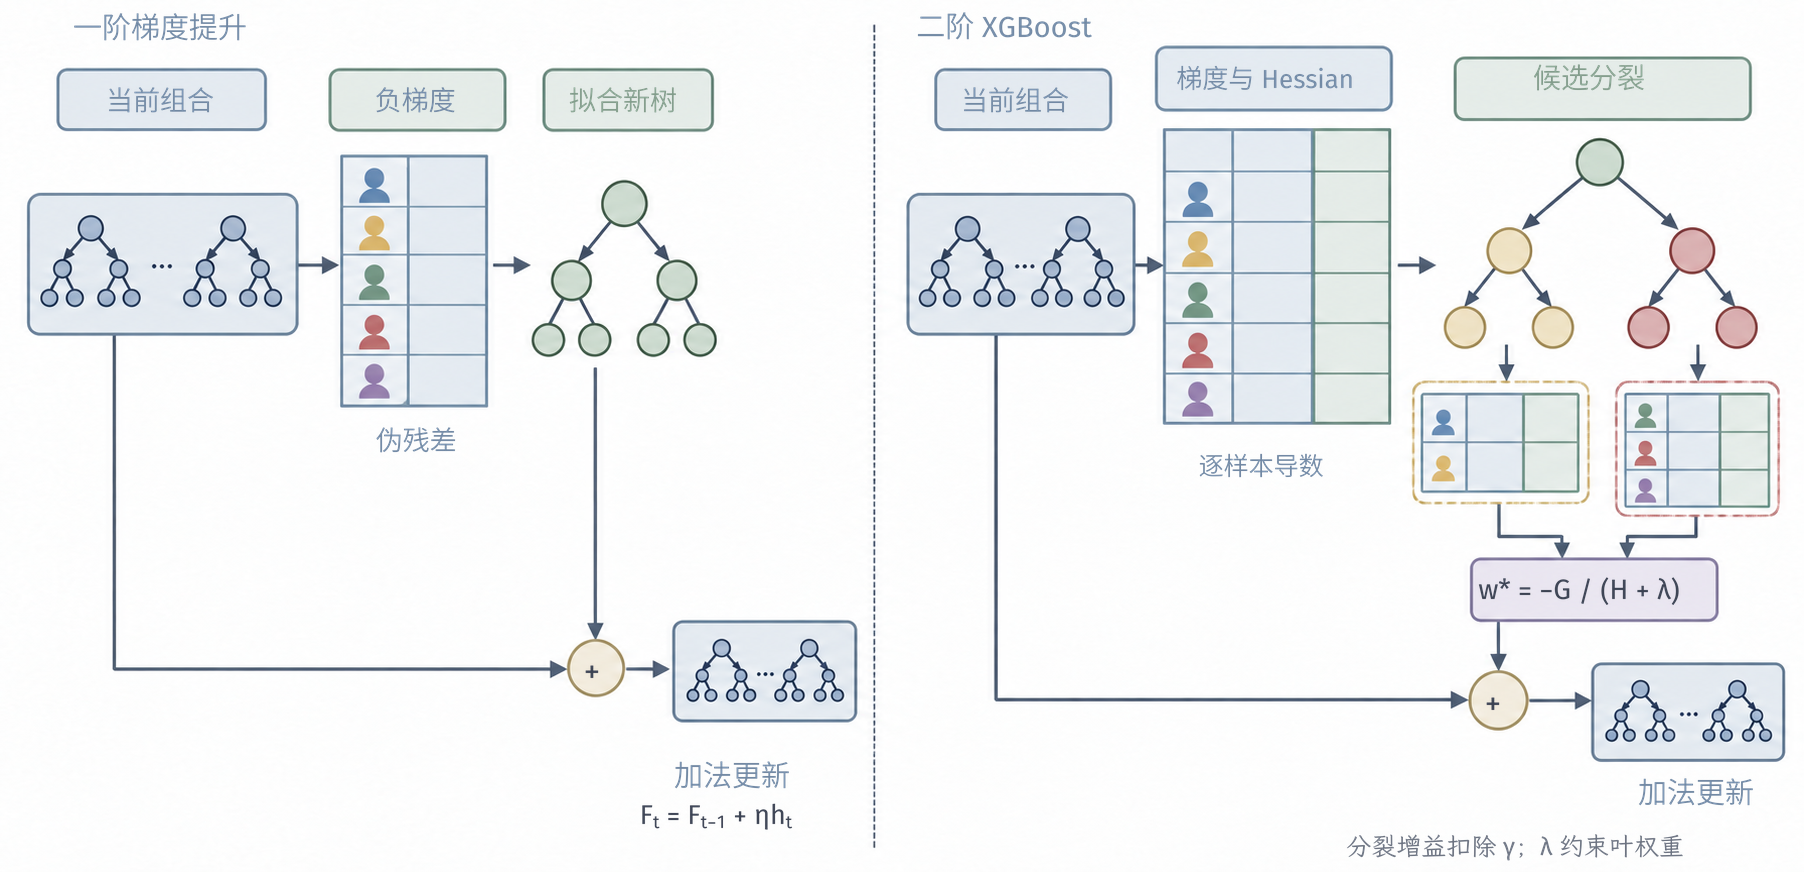
\includegraphics[width=152.739mm]{figures/03-models/01-classic-models/generated/ensemble-gradient-xgboost/figure.png}
  \caption{梯度提升与XGBoost中的本轮修正。左图中，损失对当前预测的负梯度形成伪残差，新成员拟合该信号后更新组合；右图中，XGBoost按候选分裂聚合一阶导与二阶导，再由同一组叶统计计算叶权重和分裂增益。图中单叶权重$w^\ast$对应正文的$v_j^\star$，$G$与$H$分别表示叶内一阶导和二阶导之和。复杂度项$\gamma T+\lambda\lVert\bm{w}\rVert_2^2/2$中的$T$为叶数，$\bm{w}$汇集各叶输出；$\lambda$限制叶权重，$\gamma$惩罚新增叶。该图展示当前候选树的局部评分。}
  \label{fig:ensemble-gradient-xgboost}
\end{figure*}

精确分裂搜索遍历排序后的候选特征值；近似搜索则先用带权分位数草图构造候选切分，再汇总梯度统计。稀疏感知搜索为缺失值学习默认方向，列采样减少每轮需要检查的特征。块式存储、缓存感知访问、并行统计和外存计算改变的是实现代价，不改变式\eqref{eq:ensemble-xgboost-objective}所定义的学习对象。这些设计在特定硬件和数据规模上的时间收益可通过完整训练测量确认。

\subsection{LightGBM}
\label{sec:ensemble-lightgbm}

逐值分裂搜索需要遍历候选取值，样本和特征增多会扩大这一工作量。\term{LightGBM}以直方图训练为基础，把连续特征映射到有限个桶，并在桶级别累计梯度和曲率。构造直方图仍要访问节点样本，但候选分裂只需扫描桶；已知父节点和一个子节点的直方图时，还可以用差分得到另一个子节点的统计量。分桶减少存储和候选数，也引入离散化误差。

树的生长顺序进一步改变计算分配。按层生长同时扩展某一深度上的叶，按叶生长则每次选择当前增益最大的叶继续分裂。在相同叶数下，后者把容量集中到训练目标下降较大的局部区域，可能形成深度不均衡的树。叶数、最小叶样本量和深度共同限制这种局部扩展，训练收益再由验证或测试检查其样本外效果。

LightGBM论文进一步提出两种针对大规模数据的近似。\term{单边梯度采样}（gradient-based one-side sampling, GOSS）保留绝对梯度较大的样本，从绝对梯度较小的样本中随机抽取一部分，并在分裂统计中重新加权后者。例如，在小梯度组内等概率抽取一半样本，就把被抽中者对梯度和的贡献乘二，以补偿未采样部分。一般地，样本以概率$p>0$被保留时，其贡献乘以$1/p$；给定本轮梯度和候选分区，这种逆包含概率加权可无偏估计相应的梯度和，平方、比值及择优得到的增益则是非线性量，其偏差需另行分析。

\term{互斥特征捆绑}（exclusive feature bundling, EFB）把很少同时非零的稀疏特征编码到较少的组合特征中，近似减少有效特征数。GOSS、EFB和直方图分别减少样本统计、特征表示和阈值候选，可按各自近似对象评价误差与计算节省\scite{ke2017lightgbm}。

图\ref{fig:ensemble-lightgbm-approximations}按近似对象并列这三种机制。直方图压缩候选阈值，GOSS压缩参与分裂统计的样本，EFB压缩稀疏特征表示；这三个对象分别对应数据访问、有效特征数与候选扫描的成本。

% Flush preceding margin references before the full-width illustration.
\clearpage
\begin{figure*}[htbp]
  \centering
  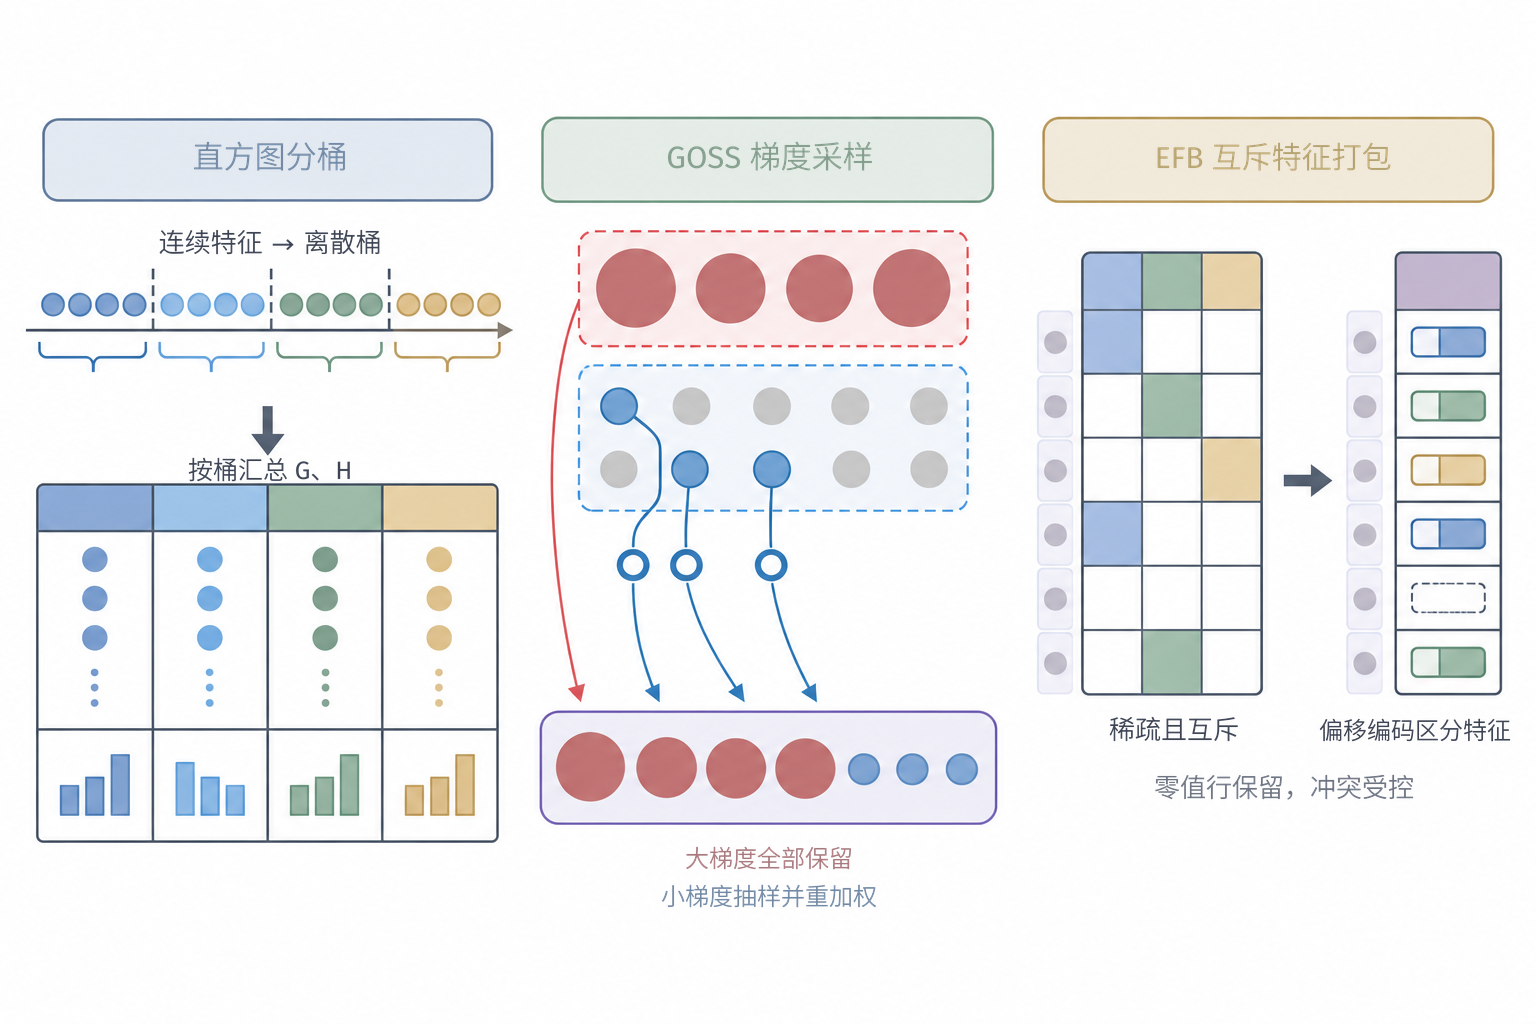
\includegraphics[width=130.048mm]{figures/03-models/01-classic-models/generated/ensemble-lightgbm-approximations/figure.png}
  \caption{LightGBM中三种作用位置不同的计算近似。直方图把连续取值映射到有限桶，GOSS保留$|g_i|$较大的样本，并抽取、重加权部分$|g_i|$较小的样本，EFB把很少同时非零的特征编码为较少的捆绑特征。图中点数、桶数与非零位置均为机制示意。}
  \label{fig:ensemble-lightgbm-approximations}
\end{figure*}

这些机制的效果依赖梯度分布、特征稀疏性、桶数、冲突处理和硬件实现。比较速度和任务损失时，需要记录数据规模、硬件、桶数与采样设置，并固定搜索预算及早停规则。论文实验的结论据此限定于相应条件。

\subsection{CatBoost}
\label{sec:ensemble-catboost}

高基数类别特征若全部展开为独热变量，会增加特征规模；把类别直接映射为整数，又会引入原本不存在的次序。另一种做法是用同类别样本的响应均值编码，但若样本自己的$y_i$参与其编码，模型就能从输入中间接看到待预测标签。训练输入含有待预测响应、部署输入却没有，这种构造差异称为\term{目标泄漏}（target leakage）。

\term{CatBoost}用随机排列建立\term{有序目标统计}（ordered target statistic）。设$c_i$为样本$i$的某个类别值，用$\pi(j)$表示样本$j$在随机排列中的位置；对当前样本只使用排列中位于它之前且类别相同的记录：
\begin{equation}
  z_i
  =
  \frac{
    \sum_{j:\,\pi(j)<\pi(i)}
    \mathbb{I}\{c_j=c_i\}y_j
    +ap
  }{
    \sum_{j:\,\pi(j)<\pi(i)}
    \mathbb{I}\{c_j=c_i\}
    +a
  }.
  \label{eq:ensemble-catboost-ordered-statistic}
\end{equation}
其中$p$是先验统计量，$a>0$控制平滑。前缀统计排除了样本自身的标签，部署时可从已观测的训练记录形成同类别统计。低频类别仍会产生较大估计波动，平滑、多个排列和类别组合需要共同考虑。

图\ref{fig:ensemble-catboost-ordered-statistics}固定当前样本的排列位置，检查哪些标签进入编码。计算当前类别$A$样本的编码时，只允许排列前缀中同为类别$A$的标签进入统计量；其他类别、当前标签和排列后缀都不参与这次编码。

\begin{figure*}[htbp]
  \centering
  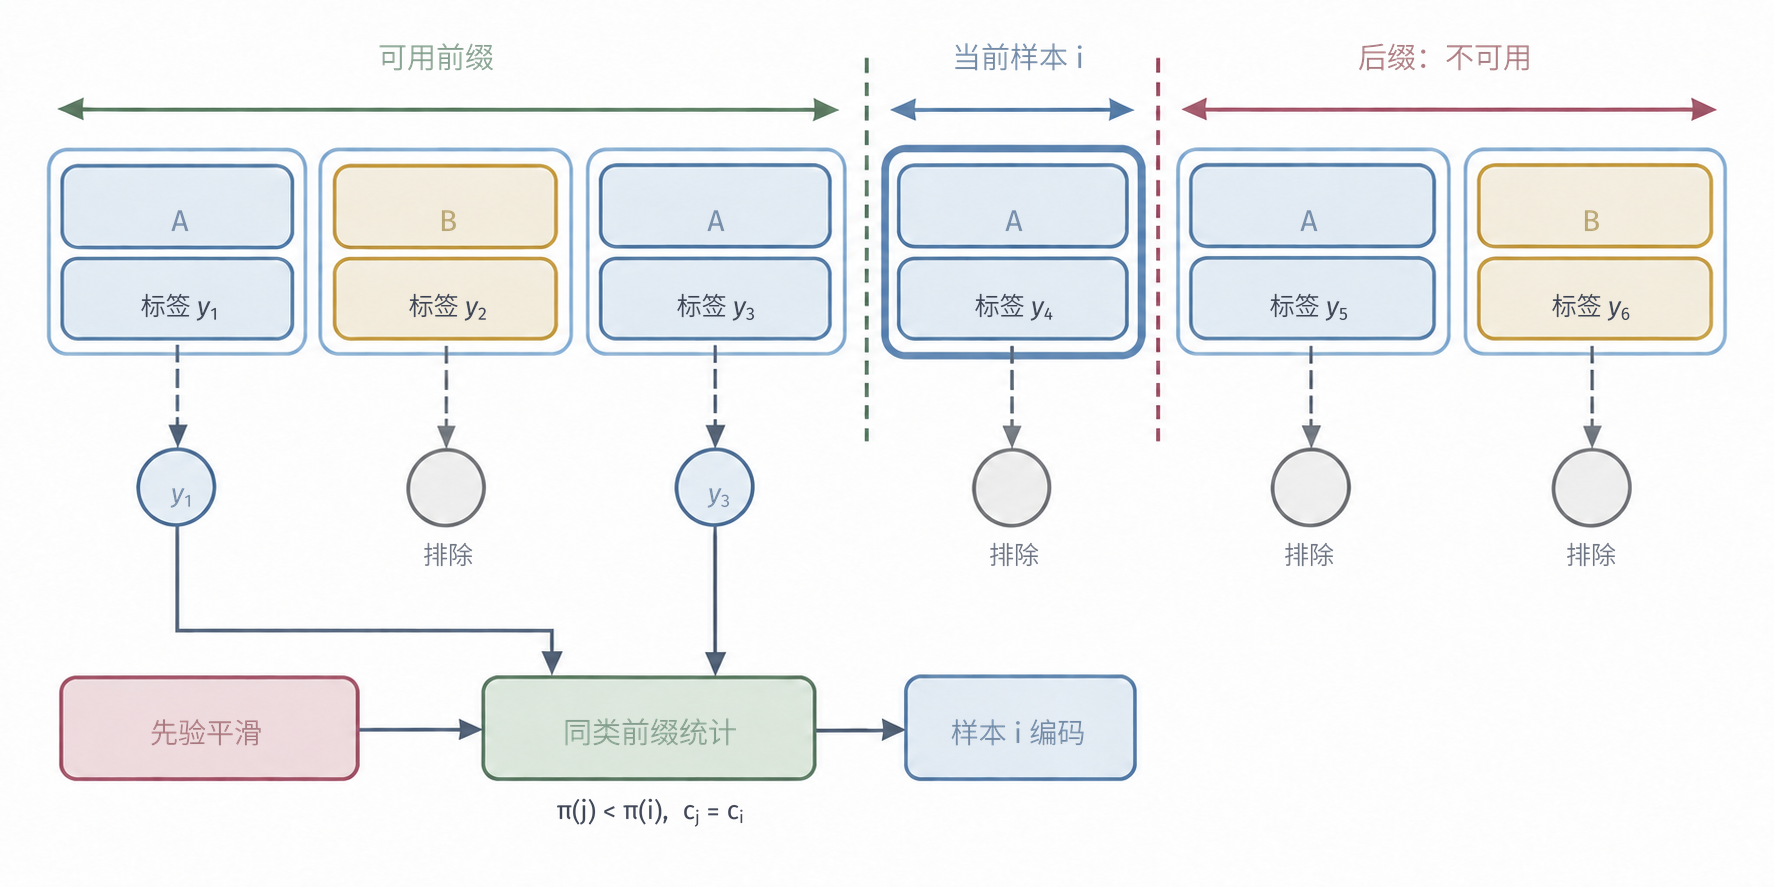
\includegraphics[width=150.199mm]{figures/03-models/01-classic-models/generated/ensemble-catboost-ordered-statistics/figure.png}
  \caption{CatBoost有序目标统计的前缀约束。这里$\pi(j)$表示样本$j$在随机排列中的位置；计算当前样本$i$的编码时，只有满足$\pi(j)<\pi(i)$且$c_j=c_i$的标签通过实线汇入统计量。其他类别、当前标签和后续记录均不连接到统计量，表示它们在本次编码中被隔离。样本索引与类别符号仅用于说明机制。}
  \label{fig:ensemble-catboost-ordered-statistics}
\end{figure*}

有序提升把相同的前缀思想用于梯度估计。计算当前样本的预测与梯度时，采用由其前缀记录拟合的相应模型，使该样本的标签与当前预测拟合分离，以减少这一重复使用带来的预测偏移。实际算法通过多个排列和前缀模型实现这一约束，训练状态与计算量也比普通单序列提升更复杂\scite{prokhorenkova2018catboost}。

CatBoost常使用\term{对称树}（symmetric tree），即同一深度的所有节点采用相同分裂条件。深度为$d_{\mathrm{tree}}$的完整对称树至多有$2^{d_{\mathrm{tree}}}$片叶，路径可以编码为固定长度的二进制选择。这种结构便于批量预测，也限制了单棵树可表达的分区形状。类别编码改变输入，有序提升改变梯度估计所用模型，对称树限制分区结构；三者的收益与代价应按各自对象评价。

\subsection{模型对比与总结}
\label{sec:ensemble-boosting-comparison}

表\ref{tab:ensemble-boosting-comparison}先固定共同的序贯加法结构，再比较各方法修改哪一层。AdaBoost由加权分类错误生成样本权重；GBM由损失梯度生成伪残差；XGBoost对正则化树目标作二阶近似；LightGBM进一步压缩分裂统计的计算；CatBoost重点处理类别统计与序贯估计中的目标泄漏。具体系统可同时使用多种训练选项，表中按代表机制比较，实际配置仍需单独记录。

\begin{table*}[htbp]
  \centering
  \small
  \begin{tabularx}{\linewidth}{@{}>{\raggedright\arraybackslash}p{19mm}*{6}{>{\raggedright\arraybackslash}X}@{}}
    \toprule
    方法 & 本轮修正信号 & 典型成员 & 目标近似 & 树生长或分裂 & 类别特征重点 & 主要约束 \\
    \midrule
    AdaBoost & 加权错分 & 树桩或浅分类树 & 指数损失下的解析更新 & 由成员算法决定 & 需另行编码 & 对持续错分记录敏感 \\
    GBM／GBDT & 负梯度伪残差 & 回归树 & 一阶函数方向与叶内优化 & 通常贪心树生长 & 需随实现处理 & 学习率、轮数与树复杂度耦合 \\
    XGBoost & 一阶导与二阶导 & 正则化回归树 & 二阶局部目标 & 精确或分位数候选；稀疏默认方向 & 依实现与版本而定 & 轮次串行，近似与系统配置影响成本 \\
    LightGBM & 桶级梯度统计 & 直方图回归树 & 通常使用二阶统计 & 按叶生长；直方图候选 & 支持类别分组，机制依实现 & 分桶、GOSS与EFB引入近似条件 \\
    CatBoost & 有序统计与有序梯度 & 对称树 & 梯度或二阶统计 & 同层共享分裂条件 & 有序目标统计与组合 & 多排列和前缀状态增加训练成本 \\
    \bottomrule
  \end{tabularx}
  \caption{Boosting代表方法的机制比较。GBM是一般框架，GBDT指使用回归树成员的实例；XGBoost、LightGBM和CatBoost是树提升的具体模型与系统，均属于Boosting框架的具体构造。}
  \label{tab:ensemble-boosting-comparison}
\end{table*}

% 跨栏表之后的扩展段需与三篇完整出处共同容纳，不能只按正文行数分页。
\Needspace{23\baselineskip}
随机梯度提升在每轮使用训练子样本，DART随机暂时移除部分已有树后计算修正，LogitBoost则从加法Logistic回归推导更新\scite{friedman2002stochastic,rashmi2015dart,friedman2000adaboost}。三种扩展分别改变抽样、当前组合及损失近似。Boosting能够沿训练目标定向增加容量，却仍采用预先规定的加法组合形式；若已有成员来自不同模型族，并希望从它们的样本外表现中学习组合方式，就进入Stacking的范围。

\section{基于Stacking的集成}
\label{sec:ensemble-stacking}

前两类方法在成员训练机制中规定了聚合方式。已有线性、近邻、森林或提升树等候选时，也可以将其预测组成新特征，学习这些特征怎样共同解释响应。\term{Stacking}（stacked generalization，堆叠）采用这种两层结构：基学习器产生一级预测，\term{元学习器}（meta-learner）把这些预测映射为最终输出\scite{wolpert1992stacked,breiman1996stacked}。

\subsection{Stacking}
\label{sec:ensemble-stacking-model}

\subsubsection{为什么不能直接使用训练内预测}

设第$m$个成员模型为$h_m$。若直接在完整训练集上拟合$h_m$，再把$h_m(\bm{x}_i)$作为样本$i$的元特征，元学习器看到的是成员对自身训练数据的预测。一个容量很大的成员可能近乎记住训练标签，元学习器便会高估它在新样本上的可靠性。训练内预测由已使用当前标签的成员产生，部署预测则面向未见标签的输入；元学习器需要面对后者的生成条件。

Stacking通常用交叉验证生成\term{折外预测}（out-of-fold prediction, OOF prediction）。把训练样本划分为$K$个互不相交的折$V_1,\ldots,V_K$。对每个成员类型$m$和每个折$k$，只用$D_n\setminus V_k$训练临时模型$h_m^{(-k)}$，再预测$V_k$中的样本。若样本$i$属于$V_{k(i)}$，元特征定义为
\begin{equation}
  z_{i,m}
  =
  h_m^{(-k(i))}(\bm{x}_i).
  \label{eq:ensemble-oof-feature}
\end{equation}
把所有成员的折外预测拼成$\bm{z}_i=(z_{i,1},\ldots,z_{i,M})^{\top}$，再由元学习算法$\mathcal{G}$训练
\[
  g=\mathcal{G}\!\left(\{(\bm{z}_i,y_i)\}_{i=1}^{n}\right).
\]
对每个样本，临时成员的拟合数据排除了它所在的折，其标签只在后续元学习器训练中使用。图\ref{fig:ensemble-stacking-oof}展示了折外矩阵的形成过程。

\begin{figure*}[htbp]
  \centering
  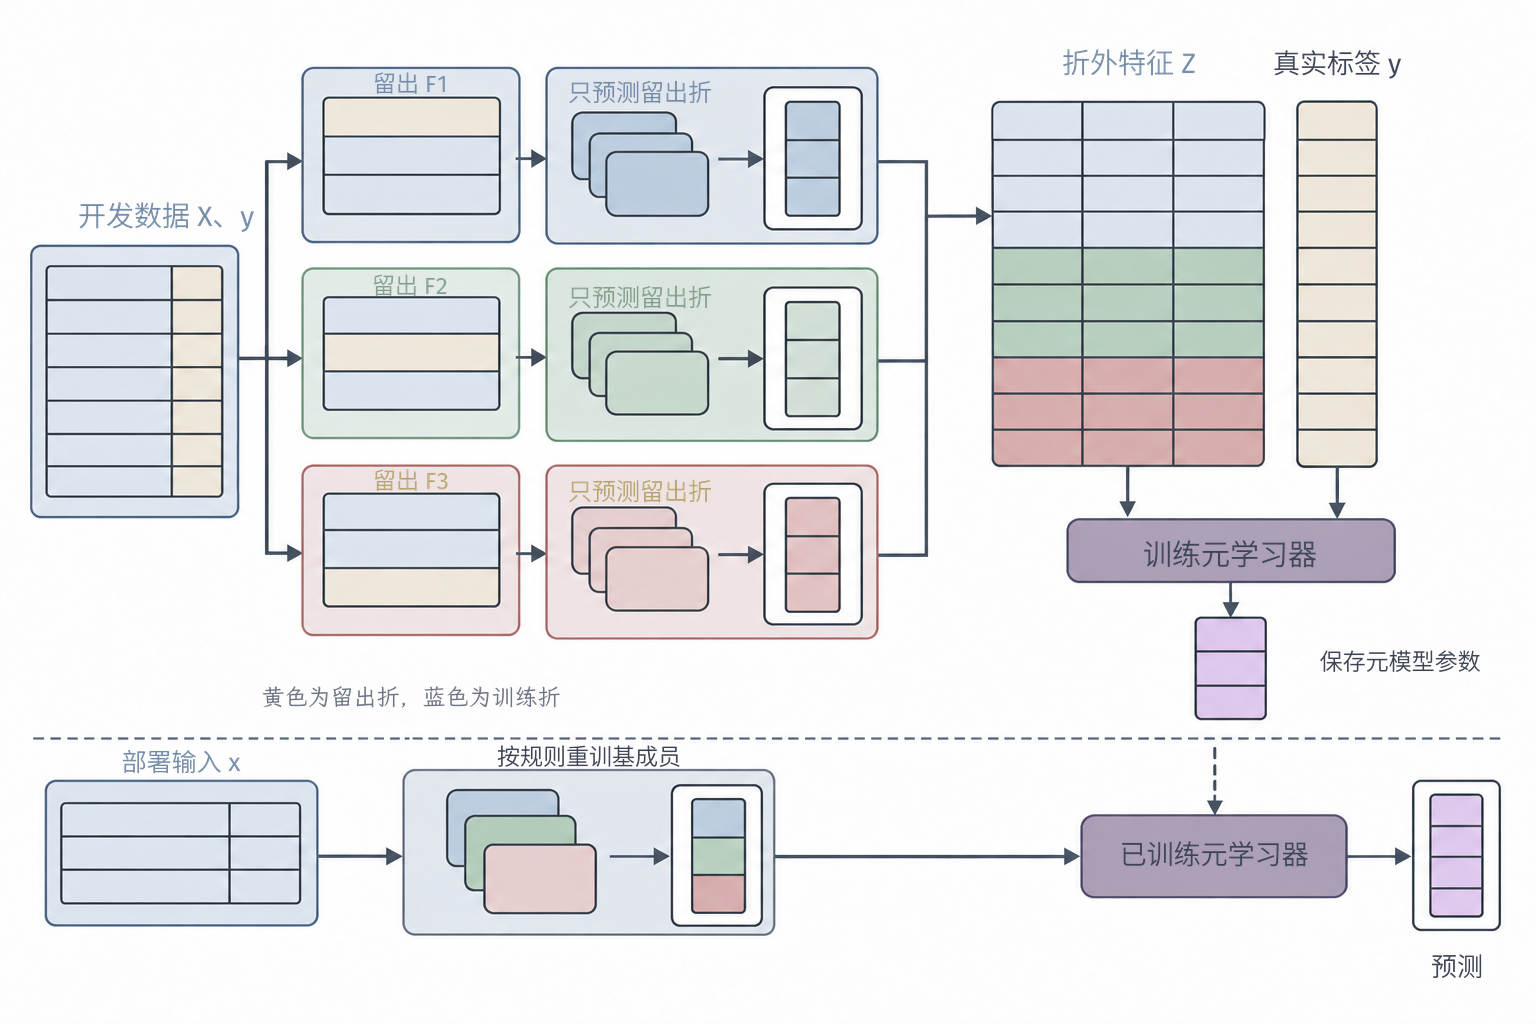
\includegraphics[width=130.048mm]{figures/03-models/01-classic-models/generated/ensemble-stacking-oof/figure.png}
  \caption{三折Stacking的折外特征构造。每一折轮流作为留出折，临时成员只在其余两折训练，并为留出折产生预测；拼接三次预测得到完整折外矩阵$\bm{Z}$，元学习器以$\bm{Z}$为输入并使用对应标签拟合。部署阶段的基成员还需按预先规定的方式重训或保留。}
  \label{fig:ensemble-stacking-oof}
\end{figure*}

分类成员若输出$C$维概率向量，一个成员通常贡献$C$列元特征；二分类时也可以只保留一个类别概率。类别硬判断省去了得分中的排序或置信信息，不同成员的得分还可能采用不同尺度。元训练与部署使用一致的输出形式，正则化再控制尺度及相关预测对组合的影响。

\subsubsection{部署模型与全量训练集重训}

折外矩阵用于训练元学习器，但部署时还需要能预测新输入的基成员。一种做法是在完整训练集上重新拟合每类基学习器$\widehat{h}_m$，预测
\[
  \widehat{y}
  =
  g\!\left(
    \widehat{h}_1(\bm{x}),\ldots,\widehat{h}_M(\bm{x})
  \right).
\]
全量重训利用全部开发数据，但训练规模增加可能改变预测分布，元学习器训练时只看过较小训练集产生的输出。也可保留各折成员，先平均它们对新输入的预测，再送入元学习器；这样沿用折内模型，同时增加了存储与推理次数。两方案的输入分布差异仍由完整验证检验。

部署方案确定后，需要评价基成员与元学习器共同形成的预测流程。基学习器的特征处理、类别编码和超参数搜索必须在相应训练折内完成。若先用全部数据选择特征或编码，再只把模型拟合放进交叉验证，信息仍可能从留出折进入元特征。

\subsection{Blending}
\label{sec:ensemble-blending}

\term{Blending}通过一次留出构造元特征，减少交叉验证的重复拟合。将可用于开发的数据分为基训练集$D_{\mathrm{base}}$和组合训练集$D_{\mathrm{blend}}$；基成员只在$D_{\mathrm{base}}$上拟合，对$D_{\mathrm{blend}}$产生预测，元学习器再以这些预测和对应标签训练。每个基成员只需完成一次用于元特征的拟合，流程比完整Stacking短。

训练数据由两层分用：基成员在$D_{\mathrm{base}}$拟合，元学习器只使用$D_{\mathrm{blend}}$的预测与标签。划分较小时，元学习器估计不稳定；划分较大时，基成员训练信息减少。多次随机划分并平均可以减小单次划分的偶然性，但它重新引入多次训练，已经不再具有单次Blending的全部成本优势。

部署时若把$D_{\mathrm{blend}}$加入基成员重新训练，基预测分布可能相对元学习器训练时发生变化；若不加入，则没有充分利用已有标签。重训方式因此属于模型配置，需要先确定，再用未参与选择的数据评价实际组合。

\subsection{受约束线性Stacking}
\label{sec:ensemble-constrained-linear-stacking}

若希望以较少参数学习成员贡献，可以在回归折外矩阵$\bm{Z}\in\mathbb{R}^{n\times M}$上学习线性组合
\begin{equation}
  (\widehat{b},\widehat{\bm{w}})
  \in
  \argmin_{b,\bm{w}}
  \frac{1}{n}
  \sum_{i=1}^{n}
  \ell\!\left(
    y_i,
    b+\bm{w}^{\top}\bm{z}_i
  \right)
  +\lambda\lVert\bm{w}\rVert_2^2.
  \label{eq:ensemble-linear-stacking}
\end{equation}
权重约束控制组合允许的尺度和方向。在$b=0$时，仅要求$w_m\geq0$得到非负线性组合，仍可能放大预测；仅要求$\sum_mw_m=1$得到仿射组合，仍可因负权重而外推。只有同时满足$b=0$、$w_m\geq0$和$\sum_mw_m=1$，才是成员预测的凸组合，输出必定位于成员预测的凸包内。非负约束排除了成员之间的正负抵消，归一化进一步限制整体尺度；有效校正若需要负权重或截距，约束会缩小候选类并增加逼近误差。

权重大小同时受输出尺度、成员相关性和损失函数影响。两个成员预测近乎相同，线性模型可以在它们之间任意分配相近作用；一个成员输出的数值范围更大，也会改变未标准化正则项下的权重。估计权重反映给定尺度、相关性与损失下的联合拟合，而非成员独立贡献。对同一类别集合上的概率向量，使用同一组满足上述凸组合条件的权重逐类组合，结果保持概率单纯形约束，样本外校准再检查概率与实际频率的对应。

\subsection{Super Learner}
\label{sec:ensemble-super-learner}

\term{Super Learner}把候选学习器库、交叉验证风险与组合权重放进一个明确程序。给定预先规定的候选库和损失，先生成每个候选的折外预测，再在指定组合类中选择交叉验证风险较小的组合；组合类可以是最佳单成员、非负线性组合或其他受控元模型。

在独立同分布、损失有界或满足相应矩条件、候选库与交叉验证方案受控等条件下，Super Learner的理论结果把其风险与候选组合类中的oracle风险联系起来：样本量增加时，交叉验证选择的组合能够渐近接近该库中最优候选或最优组合的风险\scite{vanderlaan2007superlearner}。oracle在预先给定的候选库、组合类和损失中取最优，其范围由这些设计确定。

这一比较依赖三类信息：候选库能提供什么预测，折外损失能多准确地估计目标风险，以及元模型复杂度是否得到样本支持。渐近接近oracle与有限样本中的实际改进需分别检查。若数据存在时间、群组或空间依赖，交叉验证划分还必须与部署时的新样本定义一致。

\subsection{模型对比与总结}
\label{sec:ensemble-stacking-comparison}

表\ref{tab:ensemble-stacking-comparison}比较Stacking家族的元特征来源与组合约束。标准Stacking和Super Learner都依赖折外预测；Blending以一次留出降低训练次数；受约束线性Stacking通过限制权重控制组合层容量。模型名称之外，还应记录预处理、基模型重训和元输出类型，否则无法复现实际预测链路。

\begin{table*}[htbp]
  \centering
  \small
  \begin{tabularx}{\linewidth}{@{}>{\raggedright\arraybackslash}p{25mm}*{5}{>{\raggedright\arraybackslash}X}@{}}
    \toprule
    方法 & 元特征来源 & 数据利用 & 组合规则 & 主要成本 & 主要风险 \\
    \midrule
    Stacking & $K$折折外预测 & 每个样本都产生元特征 & 可线性或非线性 & 每类成员需多次折内拟合 & 折外流程不完整造成泄漏 \\
    Blending & 固定留出集预测 & 元学习器只用留出集 & 可线性或非线性 & 基成员用于元特征时只拟合一次 & 划分敏感与重训分布变化 \\
    受约束线性Stacking & 通常为折外预测 & 与所用划分一致 & 非负、和为一或正则化线性组合 & 组合层较轻量 & 约束可能排除有效校正 \\
    Super Learner & 交叉验证预测与风险 & 由交叉验证方案决定 & 在预定库和组合类中选择 & 候选库越大，训练与选择成本越高 & oracle范围和有限样本被夸大 \\
    \bottomrule
  \end{tabularx}
  \caption{Stacking及其代表性变体。表中“数据利用”描述元学习器训练阶段；部署前是否用完整开发数据重训基成员，还需作为流程的一部分单独规定。}
  \label{tab:ensemble-stacking-comparison}
\end{table*}

多层Stacking把一层折外输出继续交给下一层，每增加一层都要重新保证当前样本没有通过上游拟合泄漏到本层特征。输入相关的门控组合则让权重随$\bm{x}$变化，它与第\ref{sec:ensemble-dynamic-selection}节的动态成员选择相邻，也与神经网络中的混合专家相接。它们增加了表达能力，同时扩大了数据划分、模型存储和调试成本；增加层数需要在相同数据与预算下取得新增预测收益，才能支持相应成本。

\section{成员选择与集成简化}
\label{sec:ensemble-selection-compression}

Bagging、Boosting和Stacking先回答怎样形成组合。部署时，多成员推理可能超出内存或延迟预算，一些成员也可能只在局部输入上有用。简化集成有三种不同目标：为所有输入固定一个较小成员子集，针对当前输入临时选择成员，或训练一个新的紧凑模型替代原集成。前两种方法保留部分原成员，第三种方法改变了部署模型。

图\ref{fig:ensemble-selection-compression}沿部署对象区分这三种目标。静态选择把成员池缩成一个固定子集，动态选择保留成员池并让路由依赖当前输入，紧凑化则把完整集成的行为转移到新模型。资源评价据此包括被部署模型以及选择或路由计算。

\begin{figure*}[htbp]
  \centering
  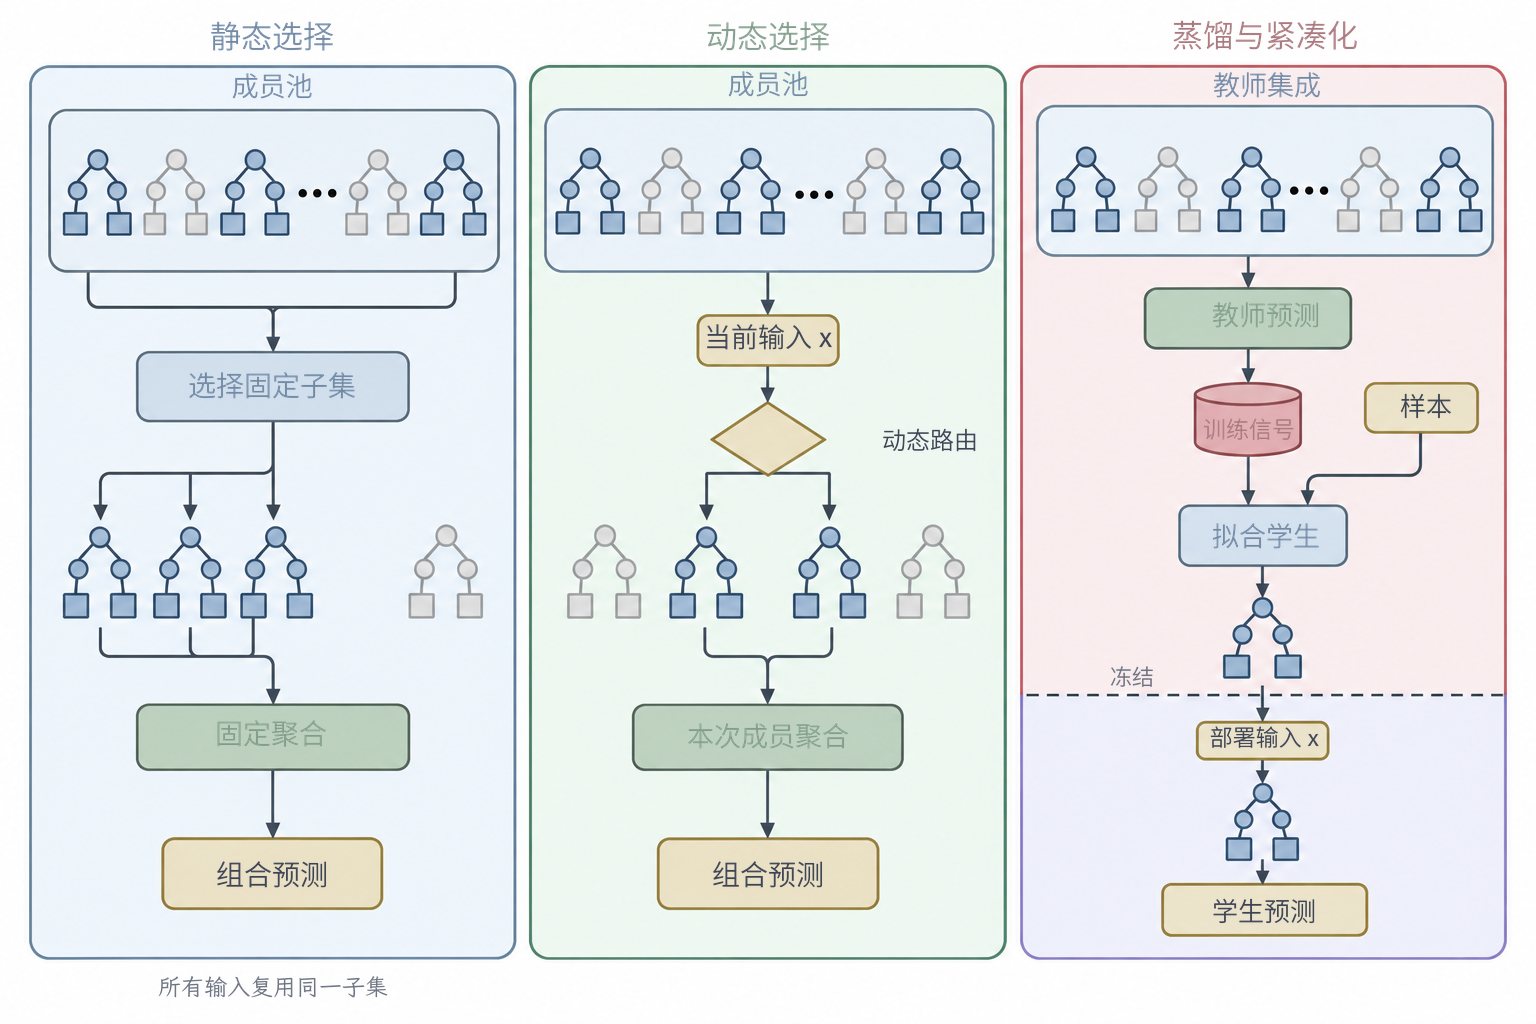
\includegraphics[width=130.048mm]{figures/03-models/01-classic-models/generated/ensemble-selection-compression/figure.png}
  \caption{静态成员选择、动态成员选择与紧凑化改变的部署对象。静态选择为所有输入保留同一成员子集；动态选择根据输入改变运行成员或组合权重；紧凑化训练并部署新的学生模型。三种路径改变的计算对象不同，成本需沿各自完整路径测量。}
  \label{fig:ensemble-selection-compression}
\end{figure*}

\subsection{静态成员选择}
\label{sec:ensemble-static-selection}

\term{静态成员选择}（static ensemble selection）给定已经训练好的候选池$\{h_1,\ldots,h_M\}$，选择一个对所有未来输入都相同的子集$S\subseteq\{1,\ldots,M\}$。若$\mathcal{L}_{\mathrm{val}}(S)$表示该子集按指定规则组合后的验证损失，可以写成
\begin{equation}
  \widehat{S}
  \in
  \argmin_{S\subseteq\{1,\ldots,M\}}
  \mathcal{L}_{\mathrm{val}}(S)
  +\lambda_1|S|
  +\lambda_2 C(S),
  \label{eq:ensemble-static-selection}
\end{equation}
其中$\lambda_1,\lambda_2\geq0$，$|S|$控制成员数，$C(S)$可以表示存储、单样本延迟或其他部署成本。成员池包含指数多个子集，实际可用排序、逐个加入或删除等方法近似搜索，并记录所得子集的验证损失与资源成本。

单成员排序忽略预测的重叠，可能同时保留许多相似模型。前向选择则评价候选加入当前组合后的损失变化，使选择依赖已有成员。允许重复选择某个成员时，重复次数还形成离散权重。基于模型库的贪心集成选择就是这种做法的代表：从一个初始组合出发，每轮加入使验证指标改善最大的候选，必要时使用多起点或装袋法减少搜索的不稳定性\scite{caruana2004ensemble}。

式\eqref{eq:ensemble-static-selection}的搜索对象为固定池中的成员子集，成员预测已经形成。若同时改变基学习算法、特征处理和超参数，搜索范围已经扩展为完整模型开发流程。候选池越大，验证集上偶然出现有利组合的机会也越多；最终测试需在该子集及其组合规则固定后进行。

分歧和误差协方差可以诊断预测关系，组合选择则以任务损失为直接依据。一个与其他成员高度不同但经常出错的模型，可能增加分歧而降低组合质量。静态选择应直接评价选定组合的输出，并在相同成员数或资源预算下与完整集成及单模型基线比较。

\subsection{动态成员选择}
\label{sec:ensemble-dynamic-selection}

静态方案让所有输入使用相同子集；若成员能力随输入区域改变，可将邻近记录上的预测结果用于当前选择。\term{动态分类器选择}（dynamic classifier selection, DCS）为每个输入选择一个成员；\term{动态集成选择}（dynamic ensemble selection, DES）选择一个成员子集或给出输入相关权重。

一种基本构造是准备独立的能力估计数据。对查询输入$\bm{x}$，在该数据中寻找非空邻域$\mathcal{N}(\bm{x})$，再以成员$m$在邻域内的正确率估计
\begin{equation}
  \widehat{c}_m(\bm{x})
  =
  \frac{1}{|\mathcal{N}(\bm{x})|}
  \sum_{i\in\mathcal{N}(\bm{x})}
  \mathbb{I}\!\left\{h_m(\bm{x}_i)=y_i\right\}.
  \label{eq:ensemble-local-competence}
\end{equation}
DCS可以选择$\widehat{c}_m(\bm{x})$最大的成员，DES则保留超过阈值的成员或按能力加权。局部正确率只是能力估计的一种方式，还可以使用输出轮廓、分类间隔或由元模型学习的能力特征\scite{woods1997localaccuracy}。

局部选择依赖邻域和能力估计两部分。邻域依赖输入表示与距离，高维或分布稀疏时，附近样本未必提供稳定的局部证据；能力估计器也可能在有限数据上过拟合。成员训练数据、能力估计数据与最终测试数据需要分开，所有标准化和邻域参数都在相应开发流程内确定。

动态选择的延迟由路由和实际运行成员共同决定。若系统必须先运行全部成员才能构造输出轮廓，再选择其中几个聚合，选择之前已经支付全部成员计算；基于输入邻域的方法还增加了检索成本。在昂贵成员运行前完成路由，才可能直接省去被跳过成员的计算；局部检索、路由和输出质量需要一并测量。

\subsection{从集成模型到紧凑模型}
\label{sec:ensemble-compression}

若原成员的最小可用子集仍超预算，可以另外训练一个新的\term{紧凑模型}（compact model），使其逼近完整集成的输入输出映射。早期模型压缩工作已经用大型集成的输出训练较小模型；知识蒸馏随后把这种教师到学生的传递扩展为常用训练形式\scite{bucilua2006compression,hinton2015distilling}。

设完整集成为教师$H$，紧凑模型为学生$s_{\bm{\theta}}$。对回归，可以组合真实响应损失与教师拟合损失：
\begin{equation}
  \min_{\bm{\theta}}
  \sum_{i=1}^{n}
  \left[
    \alpha\ell\!\left(y_i,s_{\bm{\theta}}(\bm{x}_i)\right)
    +(1-\alpha)
    \ell\!\left(H(\bm{x}_i),s_{\bm{\theta}}(\bm{x}_i)\right)
  \right],
  \label{eq:ensemble-compression-objective}
\end{equation}
其中$\alpha\in[0,1]$控制真实标签与教师输出的作用。分类时可以拟合教师的完整类别分布；温度缩放会使非最大类别之间的相对关系更容易进入训练信号，但温度、损失权重与部署概率仍须分别选择和校准。

学生训练输入可以来自原训练集、额外未标注样本或经过说明的合成样本。教师在所选输入上提供训练目标；覆盖不足的区域缺少这种监督，学生在这些区域仍可能偏离教师。学生容量过小会产生逼近误差，容量很大则可能无法达到预期资源节省。

紧凑化同时改变预测器与资源开销，可从四方面评价。预测一致性衡量学生是否复现教师输出；任务性能检查学生面对真实标签的风险；概率评价检查蒸馏后的得分是否仍可解释；资源测量确认模型大小、内存和延迟是否实际下降。训练输入上的一致性只描述局部逼近，新样本任务损失另外检查未来预测。真实标签、正则或额外数据也可使学生在部分区域改进教师预测。学生采用不同模型和训练过程，其解释、诊断及理论条件需按新模型建立。

\section{模型选择与评价}
\label{sec:ensemble-evaluation}

\subsection{成员质量、错误依赖与多样性}
\label{sec:ensemble-quality-dependence-diversity}

平均的作用可通过预测方差分析。固定输入$\bm{x}$，将训练集抽样、重采样与训练过程的随机性纳入概率空间。若$M$个成员预测具有相同方差$\sigma^2(\bm{x})$，任意两个不同成员的预测相关系数均为$\rho(\bm{x})$，则等权平均的方差为
\begin{equation}
  \operatorname{Var}\!\left[H(\bm{x})\right]
  =
  \sigma^2(\bm{x})
  \left[
    \rho(\bm{x})
    +
    \frac{1-\rho(\bm{x})}{M}
  \right].
  \label{eq:ensemble-correlated-variance}
\end{equation}
有限$M>1$时，协方差矩阵的半正定性要求$\rho(\bm{x})\geq-1/(M-1)$，因此允许一定负相关。在非负相关且增加成员时保持这一相关结构的设定下，随$M$衰减的项可解释为成员不共享的波动，$\rho(\bm{x})\sigma^2(\bm{x})$则是继续平均后保留的共同部分。式\eqref{eq:ensemble-correlated-variance}依赖等方差、等相关的简化设定，说明成员依赖对预测方差的作用；任务风险还需要结合偏差、响应噪声及相应损失。

图\ref{fig:ensemble-error-dependence}把这一差别写成成员误差的两部分。成员特有波动$u_m$在平均中可能相互抵消；若每个成员都带有共同误差$c$，增加同类成员只能继续削弱前一部分，不能消除$c$。树数控制平均次数，误差依赖控制共同部分，两者分别影响组合。

\begin{figure*}[htbp]
  \centering
  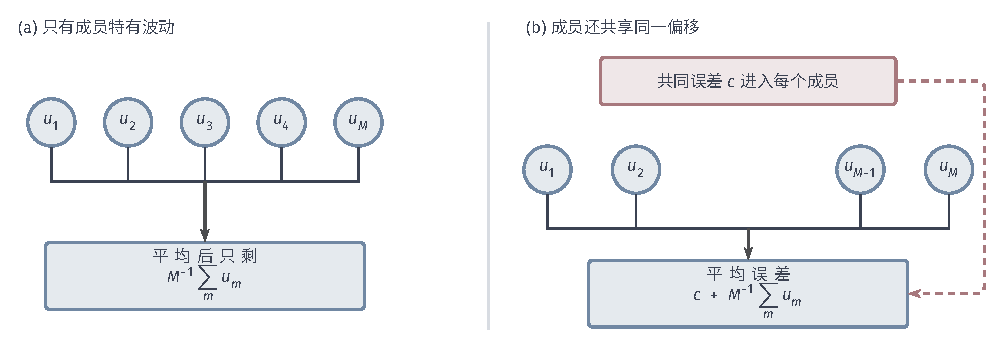
\includegraphics[width=169.000mm]{figures/04-classic-models/00-shared/tikz/ensemble-error-dependence/figure.pdf}
  \caption{成员误差依赖与平均的作用。左图表示只有成员特有波动时，平均可以随成员数增加而削弱这些波动；右图表示所有成员还共享误差$c$时，共同项仍保留在平均预测中。图中成员数量与符号只用于说明机制，不表示实测误差。}
  \label{fig:ensemble-error-dependence}
\end{figure*}

平方误差还给出另一个逐点恒等式。对非负权重$w_m$且$\sum_mw_m=1$，令$H(\bm{x})=\sum_mw_mh_m(\bm{x})$，则
\begin{equation}
  \bigl(y-H(\bm{x})\bigr)^2
  =
  \sum_{m=1}^{M}w_m\bigl(y-h_m(\bm{x})\bigr)^2
  -
  \sum_{m=1}^{M}w_m\bigl(h_m(\bm{x})-H(\bm{x})\bigr)^2.
  \label{eq:ensemble-ambiguity-decomposition}
\end{equation}
右侧第一项是成员平方误差的加权平均，第二项衡量成员围绕组合预测的分散程度，常称为歧义项\scite{krogh1995ensembles}。在成员平均误差固定时，更大的有效分散会降低组合误差；但若为了制造分散而加入很差的成员，第一项也会增大。组合的平方误差由加权成员误差与歧义项共同决定。

分类投票直接依赖各成员在哪些样本上出错。除单成员错误率外，还需记录它们的共同错误。对一对分类器，可以记录二者同时正确、只有一个正确和同时错误的样本数$n_{1,1},n_{1,0},n_{0,1},n_{0,0}$。正确性分歧率$(n_{1,0}+n_{0,1})/n$描述二者给出不同正确性结果的频率。二分类时，它等于标签分歧率；多分类时，两者同时错误也可能给出不同标签。双错率$n_{0,0}/n$直接关注共同错误；Q统计量
\[
  Q=
  \frac{n_{1,1}n_{0,0}-n_{1,0}n_{0,1}}
       {n_{1,1}n_{0,0}+n_{1,0}n_{0,1}}
\]
在分母非零时描述两种正确性结果的关联。不同指标分别描述分歧、共同错误或正确性的关联；评价集成风险时，还需结合成员准确率、组合规则与任务损失\scite{kuncheva2003diversity}。

成员差异可以从多个位置产生。改变训练样本会改变成员看到的经验分布；改变输入特征会改变可用信息；改变模型结构或超参数会改变表示与正则；改变初始化、样本顺序或分裂候选会改变优化路径。Bagging主要扰动训练样本，随机森林和Extra Trees进一步扰动特征或阈值，Stacking则允许直接组合不同模型族。这些扰动产生预测差异，差异能否减少任务错误由样本外组合损失检验。

从表达能力看，成员函数族与组合类共同规定候选预测。固定平均保留成员共有的逼近限制，加法模型逐步扩展函数，元学习器则学习成员输出之间的关系。输入相关权重还能改变不同区域的组合。

从收敛性看，Bagging增加成员数是在固定数据上逼近随机预测的平均；Boosting搜索增量并控制所选训练目标；Stacking另需求解元模型。随机平均稳定、经验目标下降及找到候选类全局最优属于不同结论，各自采用对应抽样或优化条件。

从泛化性看，成员质量、共同错误与组合复杂度都影响新样本风险。上面的方差和平方误差关系说明误差依赖的作用，独立评价再检查实际预测。折外构造、成员筛选和验证选择形成的数据依赖，也需纳入最终流程。


\subsection{方法比较}
\label{sec:ensemble-method-comparison}

表\ref{tab:ensemble-method-navigation}按成员来源、依赖和组合规则比较本章方法。相同成员数可能对应不同的模型容量与成本：Bagging的一棵深树负责完整预测，Boosting的一棵浅树只提供增量，Stacking的一个成员甚至可能是已经包含许多树的随机森林。容量与成本必须沿完整训练和预测路径衡量。

\begin{table*}[htbp]
  \centering
  \small
  \begin{tabularx}{\linewidth}{@{}>{\raggedright\arraybackslash}p{23mm}*{6}{>{\raggedright\arraybackslash}X}@{}}
    \toprule
    方法 & 成员来源 & 成员间依赖 & 组合规则 & 训练并行性 & 推理路径 & 主要失效来源 \\
    \midrule
    Bagging & 重采样或随机权重下的同类成员 & 给定原训练集后可独立生成 & 平均、投票或固定加权 & 成员间可并行 & 通常运行全部成员 & 成员稳定或共同偏差占主导 \\
    随机森林／Extra Trees & 样本、特征与阈值的随机树 & 树之间无序贯依赖 & 平均或投票 & 树间可并行 & 运行全部或选定树 & 随机化削弱单树，或相关性仍高 \\
    AdaBoost & 当前样本权重下的弱分类器 & 第$t$轮依赖前轮权重 & 训练中确定的加权投票 & 轮次串行 & 累加全部或截断成员 & 噪声记录持续获得大权重 \\
    梯度提升树 & 当前损失梯度下的回归树 & 第$t$轮依赖$F_{t-1}$ & 收缩后的加法得分 & 轮次串行，单轮可并行 & 顺序累加树输出 & 损失、轮数、树复杂度与采样失配 \\
    Stacking & 同质或异质候选模型 & 基成员可独立，元层依赖折外预测 & 学习得到的元模型 & 折与成员可部分并行 & 运行基成员后再运行元模型 & 元特征泄漏、成员冗余或元层过拟合 \\
    动态选择／紧凑化 & 已训练成员池或教师集成 & 依赖能力估计或教师输出 & 输入相关选择或新学生模型 & 依具体训练流程而定 & 选择部分成员，或只运行学生 & 路由失准、覆盖不足或逼近误差 \\
    \bottomrule
  \end{tabularx}
  \caption{集成方法的属性导航。表中成本描述方法结构，不构成固定速度排序；实际结果还受成员模型、实现、硬件、数据规模与调参预算影响。}
  \label{tab:ensemble-method-navigation}
\end{table*}

方法比较还要固定组合输出。回归均值、分位数和分布各有评价损失，分类标签、排序和概率也有不同指标。准确率的变化描述标签预测，概率校准与尾部代价则另用对应证据评价。具体指标沿用表\ref{tab:regression-evaluation-protocol}和表\ref{tab:classification-evaluation-protocol}，本节补充集成特有的数据隔离与资源记录。

\subsection{数据隔离与泄漏控制}
\label{sec:ensemble-data-isolation}

集成开发中，同一记录可能处于不同步骤的留出部分。按预测的生成方式及用途，可区分以下五类：
\begin{itemize}
  \item \term{袋外预测}来自未抽中当前样本的自助成员，用于Bagging内部诊断、置换重要性或相关构造。
  \item \term{折外预测}来自未使用当前折拟合的模型，用于训练Stacking元学习器，或为其他二阶段模型提供样本外特征。
  \item \term{能力估计预测}来自动态选择的独立开发数据，用于判断某个成员在当前输入附近是否可靠。
  \item \term{验证预测}用于选择成员数、树复杂度、学习率、组合约束、阈值与早停轮数。
  \item \term{测试预测}只在所有训练、选择、校准和部署规则冻结后产生，用于评价最终流程。
\end{itemize}
图\ref{fig:ensemble-data-isolation}把五类预测放回各自的数据路径。前四类仍处在模型开发阶段，允许影响规定范围内的诊断、二阶段训练或选择；测试预测位于流程冻结之后，只负责评价最终链路。标明生成与使用路径，可以检查当前标签是否经过拟合、选择或校准返回预测。

\begin{figure*}[htbp]
  \centering
  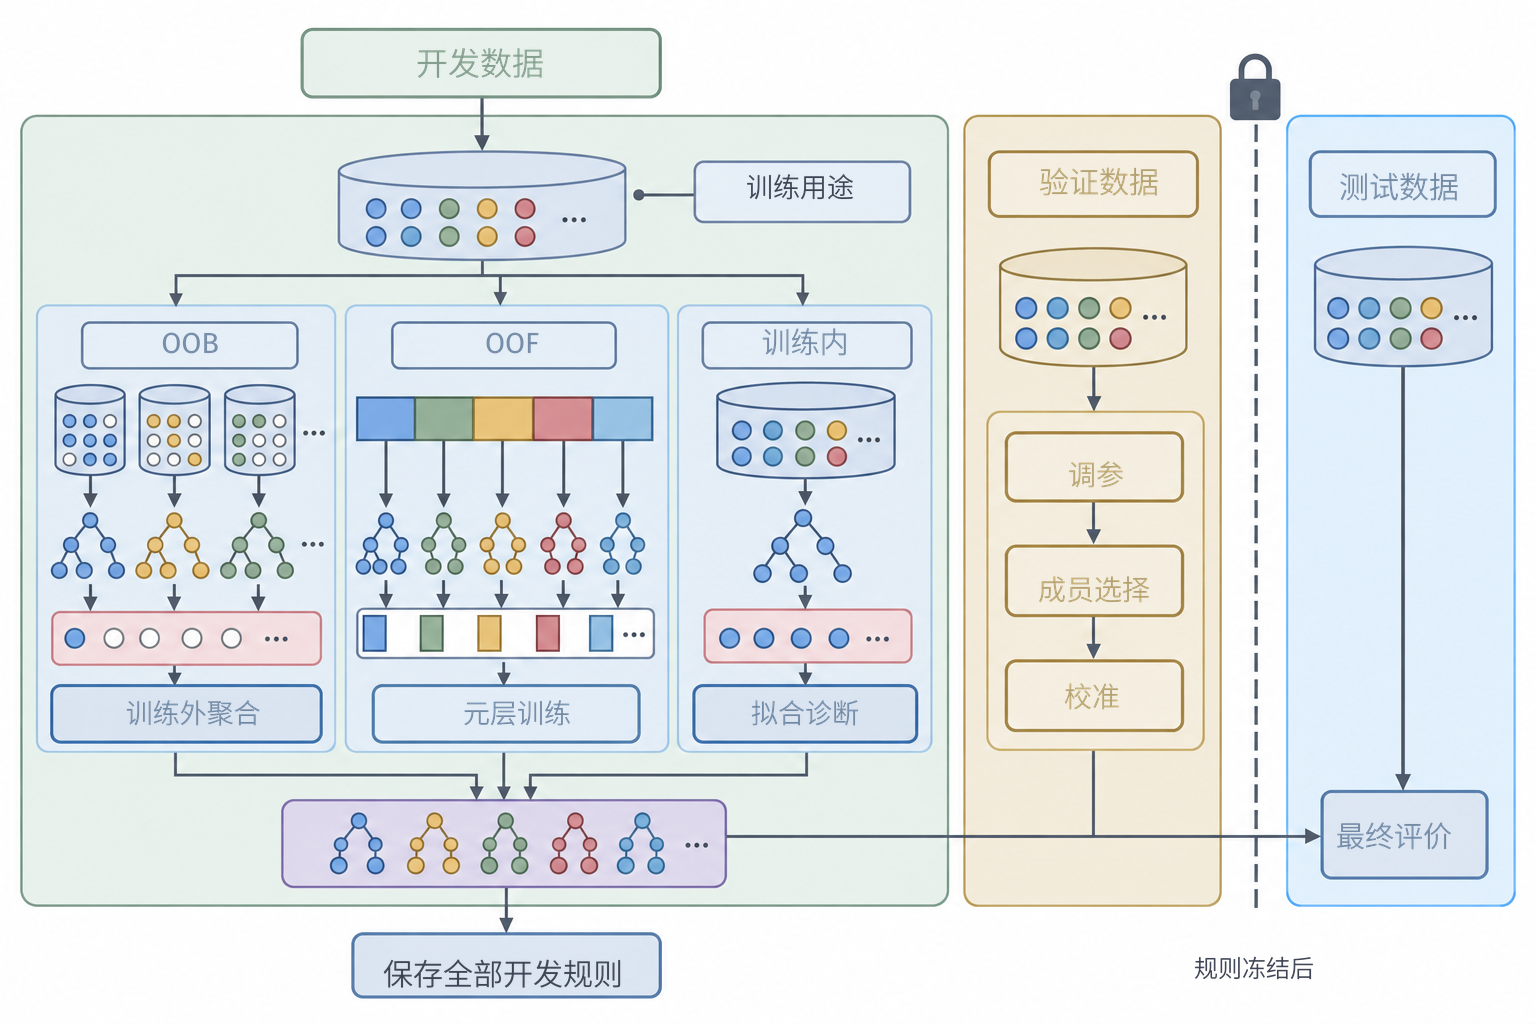
\includegraphics[width=130.048mm]{figures/04-classic-models/00-shared/generated/ensemble-data-isolation/figure.png}
  \caption{集成学习中的数据隔离与预测职责。开发阶段的预测及验证数据各有规定用途；测试阶段前的竖直分隔线表示训练、调参、筛选、校准和部署规则已经冻结。测试预测评价已经冻结的流程；图中不向开发步骤返回选择信号。}
  \label{fig:ensemble-data-isolation}
\end{figure*}

留出条件只针对产生当前预测的拟合步骤，其后用途仍会引入新的数据依赖。折外矩阵参与元学习器训练，因而不是最终测试证据；袋外误差若反复用于选择随机森林参数，也已经参与模型开发；动态能力数据若同时训练成员，会高估局部能力。

泄漏还可能发生在模型拟合之前。缺失值填补、标准化、特征选择、目标编码和降维若利用了当前留出折，就会把信息带入折外预测。基成员调参、成员池筛选、元学习器调参和概率校准也要放在正确的数据层级。需要同时比较候选成员和组合规则时，可以在外层保留最终测试集，在内层训练折中完成全部预处理、调参及折外特征构造；时间、患者、用户或设备等依赖单位则按部署边界分组划分。

样本有限时，可用嵌套交叉验证或交叉拟合复用开发记录；每个用于评价或构造元特征的预测仍须由相应留出路径产生。应记录每个预测由哪些样本训练的哪些模型产生，使元训练、选择与最终评价的角色可追溯。

\subsection{预测质量与资源成本}
\label{sec:ensemble-quality-resource}

集成结果至少要与三个基线比较：相同任务下的合理单模型、未简化的完整集成，以及满足同一资源限制的候选方法。合理单模型提供基本预测参照，完整集成检验简化损失，同预算方法检验资源取舍。成员与组合的同时记录还可解释收益来自哪一步。

对Bagging，可以同时报告代表性单成员损失、成员预测相关或双错率、集成损失以及损失随成员数的变化。对Boosting，应区分训练损失、验证轨迹和最终测试结果，并记录早停轮数。对Stacking，应比较各成员的折外表现、折外预测依赖、元模型的新增验证收益和全链路测试结果。多样性记录用于解释依赖，选型仍以任务损失及预算为依据。

输出为概率时，需要检查数值与真实频率的对应。平均可保留成员共同的过度自信，提升得分则先经适当链接转换为概率。若使用后处理校准，校准器只能接收未用于拟合该预测的数据，并要把它作为部署链路的一部分，在最终测试集上报告对数损失、Brier分数、可靠性及任务决策损失。

资源比较记录预处理、成员、组合与路由的完整计算。训练侧至少包括总计算量、墙钟时间、峰值内存、并行资源和调参次数；部署侧包括序列化模型大小、加载内存、单样本延迟、批量吞吐及预处理和路由开销。Bagging的成员训练可以并行，但推理通常运行多个成员；Boosting轮次串行，树内统计可并行；Stacking既要运行基成员，又要运行元模型。静态选择、动态选择和紧凑化是否真正节省资源，只能由端到端测量回答。

\subsection{从问题条件到候选方法}
\label{sec:ensemble-method-selection}

当单模型对训练样本、随机种子或局部分裂明显敏感，并且可以承担多个成员的存储与预测成本时，Bagging是直接候选。树成员反复依赖少数强特征时，可以进一步比较随机森林；若阈值搜索成本较高且可以接受更强的随机化，再比较Extra Trees。在固定任务上比较单树变化、成员共同错误及组合损失，可以确认这些随机化是否带来所需收益。

当任务损失能够提供有意义的逐轮修正，并且训练流程可以承担序贯依赖时，可以考虑Boosting。AdaBoost适合检查重加权分类的机制；一般损失与树成员则进入GBDT。三种树提升系统的代表机制给出不同候选条件：需要分别判断是否重视正则化二阶树目标与稀疏路径、直方图及大规模稀疏统计、或类别特征的有序统计，并在当前硬件和搜索预算下实测。

当候选模型已经产生互补的样本外预测，而且可以承担交叉验证与多模型部署成本时，Stacking提供学习式组合。固定留出只让部分样本参加元训练，折外构造可让全部开发样本产生元特征；成员高度相关时，线性约束可以限制元模型的自由度。Super Learner的理论比较范围由候选库、损失和组合类共同决定，有限样本表现再按冻结流程评价。

成员池超过部署预算时，再判断要保留什么对象。希望所有输入走同一条较短路径时采用静态成员选择；有可靠局部能力数据且路由开销可控时考虑动态选择；完整集成质量合格但任何成员子集都达不到预算时，可以训练紧凑模型。以上条件只负责缩小候选范围，最终选择据相同数据制度、调参预算与资源测量下的新样本证据确定。


\Needspace{18\baselineskip}
\section{本章小结}
\label{sec:ensemble-summary}

集成利用成员生成与组合规则改变预测误差。互补作用来自成员能够在部分输入上修正彼此的判断，共同遗漏的结构仍需改变表示或训练方式。Bagging通过样本、特征或分裂随机性构造可并行成员，再用平均或投票削弱一部分训练波动；Boosting让每轮成员依赖当前组合，沿选定损失逐步加入修正；Stacking使用折外预测训练元学习器，使组合规则本身也由数据决定。三类机制可以嵌套，但各自的数据依赖、计算路径和失效原因不同。

成员池形成后，还可以改变部署规模。静态成员选择为所有输入固定同一子集，动态成员选择针对当前输入估计局部能力，紧凑化则训练一个新模型逼近完整集成。选择保留原成员的部分计算，紧凑化则部署一个重新训练的预测器，因此其成本与误差来源需要分别评价。

最终评价针对成员训练、选择和部署规则全部固定后的预测流程。袋外预测服务于Bagging内部诊断，折外预测服务于Stacking的元特征构造，能力估计数据服务于动态选择；前述预测用于开发，最终测试再评价冻结后的完整流程。比较方法时还要固定调参预算，并同时报告任务损失、概率质量、模型大小和端到端延迟。后续神经网络模型部分将在这些共同原则上，进一步讨论由初始化、数据顺序与训练过程产生的神经网络集成。

\paragraph{扩展阅读}
Hastie等的教材从加法建模解释提升方法；Breiman的Bagging与随机森林论文说明重采样及特征随机化的作用。可选同一预测任务，比较成员误差中可被组合削弱的部分，并记录获得这一收益所需的训练与部署成本\scite{hastie2009,breiman1996bagging,breiman2001randomforests}。
